\documentclass[12pt,a4paper,oneside,french]{book}
\usepackage{mathpazo}
\usepackage{helvet}
\usepackage{courier}
\usepackage[T1]{fontenc}
\usepackage[utf8]{inputenc}
\setcounter{secnumdepth}{3}
\setcounter{tocdepth}{3}
\setlength{\parskip}{\medskipamount}
\setlength{\parindent}{0pt}
\usepackage{color}
\usepackage{babel}
\makeatletter
\addto\extrasfrench{
    \providecommand{\og}{\leavevmode\flqq~}
    \providecommand{\fg}{\ifdim\lastskip>\z@\unskip\fi~\frqq}}

\makeatother
\usepackage{amsmath}
\usepackage{amsthm}
\PassOptionsToPackage{version=3}{mhchem}
\usepackage{mhchem}
\usepackage[unicode=true,
    bookmarks=true,bookmarksnumbered=true,bookmarksopen=true,bookmarksopenlevel=2,
    breaklinks=true,pdfborder={0 0 1},backref=false,colorlinks=true]
    {hyperref}
\hypersetup{pdftitle={Théorie de Collision},
    pdfauthor={Mohamed Amine Boussoubel/Abderrahmane Labane},
    linkcolor=black,citecolor=black,urlcolor=blue,filecolor=blue,pdfpagelayout=OneColumn,pdfnewwindow=true,pdfstartview=XYZ,plainpages=false}

\makeatletter

\special{papersize=\the\paperwidth,\the\paperheight}


\usepackage{amsthm}
\usepackage{tikz, tikz-3dplot}
\usepackage{pgfplots}
\usepackage{float}
\usepackage{physics}
\usepackage{relsize}

\usetikzlibrary{calc, patterns, angles, quotes, shapes}

\pagenumbering{roman}
\let\myTOC\tableofcontents
\renewcommand\tableofcontents{
    \pdfbookmark[1]{\contentsname}{}
    \myTOC
    \cleardoublepage
    \pagenumbering{arabic}}

\renewcommand{\i}{\mathrm{i}}
\newcommand{\e}{\mathrm{e}}
\newcommand{\opr}[1]{\mathrm{\hat{#1}}}
\newcommand{\diff}{\mathrm{d}}
\newcommand{\identity}{\mathbb{1}}
\newcommand{\pvec}[1]{\vec{#1} \mkern2mu \vphantom{#1}}
\newcommand{\bigint}[2]{\mathop{\mathlarger{\int_{#1}^{#2}}}}
\newcommand{\Bigint}[2]{\mathop{\mathlarger{\mathlarger{\mathlarger{\int_{#1}^{#2}}}}}}
\newcommand{\removeintspace}{\!\!\!\!\!\!\!\!}

\DeclareMathOperator*{\res}{Res}

\theoremstyle{definition}
\newtheorem*{definition}{Définition}

\theoremstyle{definition}
\newtheorem*{example}{Example}

\theoremstyle{definition}
\newtheorem*{examples}{Examples}

\theoremstyle{remark}
\newtheorem*{remark}{Remarque}

\theoremstyle{definition}
\newtheorem*{application}{Application}

\makeatother

\begin{document}
    \title{Théorie de Collision}
    \author{}
    
    \maketitle
    \tableofcontents{}
    
    
    
    \chapter{Processus de collision en mécanique quantique}
    
    \section{Introduction}
    La plupart des découvertes en physique sont le résultat d'expériences de collision.
    
    \begin{examples}
        \leavevmode
        
        \begin{itemize}
            \item 
            Découvertes du noyau atomique par \textsc{Rutherford}.
            
            \item
            Spectroscopie nucléaire et atomique.
            
            \item
            Fission nucléaire.
            
            \item
            Découverte des particules élémentaires et leurs propriétés.
        \end{itemize}
    \end{examples}
    
    Ce chapitre sera consacré aux notions élémentaires concernant les problèmes de collision. Les résultats des expériences dans ce domain s'expriment au moyen de quantités appelées \textbf{sections efficaces}. Ces dernières sont direcement liées au comportement asymptotique des solutions stationnaires de l'équation de \textsc{Schrödinger}.
    
    \section{Déscription classique d'une collision}
    On dit qu'il y a collision entre deux ou plusieurs particules quand elles subissent une interaction mutuelle de courte durée et de courte portée. Cette collision est localisée dans le temps et dans l'espace. \\
    
    En règle générale, les forces d'interaction sont négligeables quant les particules sont suffisament éloignées. On peut donc déstingué un \textbf{avant} et un \textbf{après} la collision.
    
    \bigskip
    
    \begin{figure}[!h]
        \centering
        
        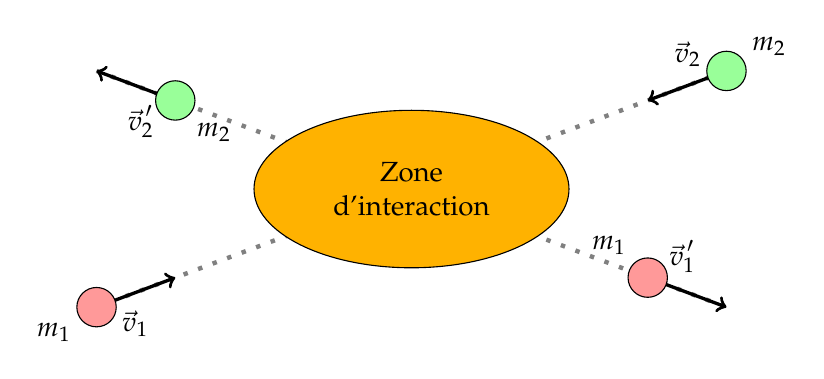
\begin{tikzpicture}
            \draw[gray, ultra thick, loosely dotted](-4, -1.5) -- (4, 1.5);
            \draw[gray, ultra thick, loosely dotted](-4, 1.5) -- (4, -1.5);
            
            \filldraw[color = black, fill = orange!60!yellow](0, 0) ellipse (2cm and 1cm);
            \node[align = center] at (0, 0) {Zone \\ d'interaction};
            
            \draw[black, very thick, ->](-4, -1.5) -- (-4 * 0.75, -1.5 * 0.75);
            \node[align = center, anchor = north west] at (-4 * 0.95, -1.5 * 0.95) {${\vec{v}}_{1}$};
            \filldraw[color = black, fill = red!40](-4, -1.5) circle (0.25cm);
            \node[align = center, anchor = north east] at (-4 * 1.05, -1.5 * 1.05) {${m}_{1}$};
            
            \draw[black, very thick, ->](4, 1.5) -- (4 * 0.75, 1.5 * 0.75);
            \node[align = center, anchor = south east] at (4 * 0.95, 1.5 * 0.95) {${\vec{v}}_{2}$};
            \filldraw[color = black, fill = green!40](4, 1.5) circle (0.25cm);
            \node[align = center, anchor = south west] at (4 * 1.05, 1.5 * 1.05) {${m}_{2}$};
            
            \draw[black, very thick, ->](4 * 0.75, -1.5 * 0.75) -- (4, -1.5);
            \node[align = center, anchor = south west] at (4 * 1.05 * 0.75, -1.5 * 1.05 * 0.75) {${\pvec{v}}_{\! 1}'$};
            \filldraw[color = black, fill = red!40](4 * 0.75, -1.5 * 0.75) circle (0.25cm);
            \node[align = center, anchor = south east] at (4 * 0.95 * 0.75, -1.5 * 0.85 * 0.75) {${m}_{1}$};
            
            \draw[black, very thick, ->](-4 * 0.75, 1.5 * 0.75) -- (-4, 1.5);
            \node[align = center, anchor = north east] at (-4 * 1.05 * 0.75, 1.5 * 1.05 * 0.75) {${\pvec{v}}_{\! 2}'$};
            \filldraw[color = black, fill = green!40](-4 * 0.75, 1.5 * 0.75) circle (0.25cm);
            \node[align = center, anchor = north west] at (-4 * 0.95 * 0.75, 1.5 * 0.85 * 0.75) {${m}_{2}$};
        \end{tikzpicture}
        
        \caption{Collision élastique de 2 particules}
    \end{figure}
    
    Connaissant les vitesses ${\vec{v}}_{i}$, on peut déduire des informations sur les vitesses ${\pvec{v}}_{\! i}'$ et vice versa.
    
    \subsection{Grandeurs conservées}
    Malgré notre connaisance partielle du problème, on peut obtenir certaines informations grâce aux lois de conservation. \\
    
    On considère que le système $\mathcal{S}$ de deux particules est isolé de l'extérieur.
    
    \begin{itemize}
        \itemsep1em
        
        \item 
        Conservation de la quantité de mouvement totale :
        \begin{equation*}
            \frac{\diff {\vec{P}}_{\mathcal{S}}}{\diff t} = {\vec{F}}^{ext} = 0, \qquad {\vec{P}}_{\mathcal{S}} = \sum_{i}^{N} {\vec{p}}_{i} = \sum_{i}^{N'} {\pvec{p}}_{\! i}' = {\pvec{P}}_{\! \mathcal{S}}'
        \end{equation*}
        
        \item
        Conservation de l'énergie totale : \\
        
        Si les forces d'interaction entre les particules dérivent d'une énergie potentielle (forces conservatives), alors l'énergie totale du système s'écrit :
        
        \begin{equation*}
            {E}_{T}^{\mathcal{S}} = {E}_{c}^{\mathcal{S}} + {E}_{p}^{\mathcal{S}} + \sum_{i}^{N} {U}_{i} = {E'}_{\!\! c}^{\mathcal{S}} + {E'}_{\!\! p}^{\mathcal{S}} + \sum_{i}^{N'} {U'}_{\!\! i} = {E'}_{\!\! T}^{\mathcal{S}}
        \end{equation*}
        
        ${E}_{c}^{\mathcal{S}}, \ {E}_{p}^{\mathcal{S}}$ et ${U}_{i}$ sont les énergies cinétique, potentielle (l'interaction entre les particules) et interne, respectivement. \\
        
        Si on néglige les interactions entre particules, on obtient :
        
        \begin{equation*}
            {E}_{c}^{\mathcal{S}} + \sum_{i}^{N} {U}_{i} = {E'}_{\!\! c}^{\mathcal{S}} + \sum_{i}^{N'} {U'}_{\!\! i}
        \end{equation*}
        
        $N$ et $N'$ est le nombre de particules avant et après la collision.
    \end{itemize}
    
    \subsection{Collision élastique}
    On dit qu'il y a collision élastique lorsque avant et après la collision on a :
    
    \begin{itemize}
        \item 
        Le nombre de particules reste constant.
        
        \item
        L'énergie interne de chaque particule reste inchangée.
    \end{itemize}
    
    \bigskip
    
    En d'autre terme, les particules ne se déforment pas et ne changent pas de nature. \\
    
    Les lois de conservation sont donc :
    
    \begin{equation*}
        {m}_{i}^{\mathcal{S}} = {m'}_{\!\! i}^{\mathcal{S}}\!\!\!, \qquad {\vec{P}}_{\mathcal{S}} = {\pvec{P}}_{\! \mathcal{S}}', \qquad {E}_{T}^{\mathcal{S}} = {E'}_{\!\! T}^{\mathcal{S}}
    \end{equation*}
    
    \begin{examples}
        \leavevmode
        
        \begin{itemize}
            \item 
            Collision entre les balles de billard.
            
            \item
            Diffusion de \textsc{Rutherford} (diffusion d'un noyau $\ce{^{4}_{2}He++}$ par un noyau positif).
        \end{itemize}
    \end{examples}
    
    \begin{figure}[!h]
        \centering
        
        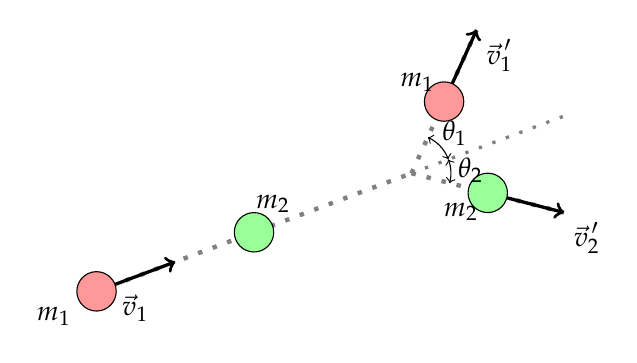
\begin{tikzpicture}
            \coordinate (origin) at (0, 0);
            \coordinate (vec_outcome_dir1) at ({cos(45 + atan(-1.5 / -4))}, {sin(45 + atan(-1.5 / -4))});
            \coordinate (vec_outcome_dir2) at ({cos(-35 + atan(-1.5 / -4))}, {sin(-35 + atan(-1.5 / -4))});
            \coordinate (end) at (4 * 0.5, 1.5 * 0.5);
            
            \draw[gray, ultra thick, loosely dotted](-4, -1.5) -- (origin);
            \draw[gray, very thick, loosely dotted](origin) -- (end);
            \draw[gray, ultra thick, loosely dotted](origin) -- ($(vec_outcome_dir1) + (vec_outcome_dir1)$);
            \draw[gray, ultra thick, loosely dotted](origin) -- ($(vec_outcome_dir2) + (vec_outcome_dir2)$);
            
            \draw[black, very thick, ->](-4, -1.5) -- (-4 * 0.75, -1.5 * 0.75);
            \node[align = center, anchor = north west] at (-4 * 0.95, -1.5 * 0.95) {${\vec{v}}_{1}$};
            \filldraw[color = black, fill = red!40](-4, -1.5) circle (0.25cm);
            \node[align = center, anchor = north east] at (-4 * 1.05, -1.5 * 1.05) {${m}_{1}$};
            
            \filldraw[color = black, fill = green!40](-4 * 0.5, -1.5 * 0.5) circle (0.25cm);
            \node[align = center, anchor = south west] at (-4 * 0.5 * 1.05, -1.5 * 0.4 * 1.05) {${m}_{2}$};
            
            \draw[black, very thick, ->](vec_outcome_dir1) -- ($(vec_outcome_dir1) + (vec_outcome_dir1)$);
            \node[align = center, anchor = north west] at ($(vec_outcome_dir1) + (vec_outcome_dir1)$) {${\pvec{v}}_{\! 1}'$};
            \filldraw[color = black, fill = red!40](vec_outcome_dir1) circle (0.25cm);
            \node[align = center, anchor = south east] at (vec_outcome_dir1) {${m}_{1}$};
            
            \draw[black, very thick, ->](vec_outcome_dir2) -- ($(vec_outcome_dir2) + (vec_outcome_dir2)$);
            \node[align = center, anchor = north west] at ($(vec_outcome_dir2) + (vec_outcome_dir2)$) {${\pvec{v}}_{\! 2}'$};
            \filldraw[color = black, fill = green!40](vec_outcome_dir2) circle (0.25cm);
            \node[align = center, anchor = north east] at (vec_outcome_dir2) {${m}_{2}$};
            
            \pic[draw, <->, "${\theta}_{1}$", angle eccentricity = 1.5] {angle = end--origin--vec_outcome_dir1};
            \pic[draw, <->, "${\theta}_{2}$", angle eccentricity = 1.5] {angle = vec_outcome_dir2--origin--end};
        \end{tikzpicture}
        
        \caption{Collision de 2 particules, ${m}_{2}$ est au repos}
    \end{figure}
    
    Les lois de conservation donnent :
    
    \begin{equation*}
    \begin{cases}
        {m}_{1} {\vec{v}}_{1} = {m}_{1} {\pvec{v}}_{\! 1}' + {m}_{2} {\pvec{v}}_{\! 2}' \\
        \frac{1}{2} {m}_{1} {v}_{1}^{2} = \frac{1}{2} {m}_{1} {v'}_{\!\! 1}^{2} + \frac{1}{2} {m}_{2} {v'}_{\!\! 2}^{2}
    \end{cases}
    \end{equation*}
    
    \subsection{Collision inélastique}
    On dit qu'une collision est inélastique lorsqu'une  partie de l'énergie cinétique initiale du système s'est transformée en d'autre formes d'énergie. \\
    
    La collision s'accompagne alors d'une variation d'énergie interne et/ou d'une modification du nombre de particules. Certaines peuvent être créées pas fragmentation ou par équivalence masse-énergie.
    
    \begin{example}
        Réaction chimique.
    \end{example}
    
    Lorsqu'on laisse tomber une pâte à modeler, celle-ci ne rebondit pas, toute l'énergie cinétique acquise par la boule avant l'impact est convertie en énergie interne d'où une déformation et un échauffement du projectile.
    
    \begin{figure}[!h]
        \centering
        
        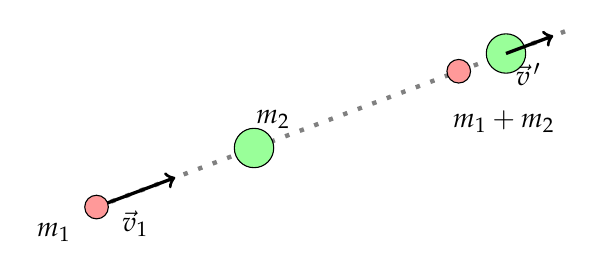
\begin{tikzpicture}
            \coordinate (origin) at (0, 0);
            \coordinate (end) at (4 * 0.5, 1.5 * 0.5);
            
            \draw[gray, ultra thick, loosely dotted](-4, -1.5) -- (end);
            
            \draw[black, very thick, ->](-4, -1.5) -- (-4 * 0.75, -1.5 * 0.75);
            \node[align = center, anchor = north west] at (-4 * 0.95, -1.5 * 0.95) {${\vec{v}}_{1}$};
            \filldraw[color = black, fill = red!40](-4, -1.5) circle (0.15cm);
            \node[align = center, anchor = north east] at (-4 * 1.05, -1.5 * 1.05) {${m}_{1}$};
            
            \filldraw[color = black, fill = green!40](-4 * 0.5, -1.5 * 0.5) circle (0.25cm);
            \node[align = center, anchor = south west] at (-4 * 0.5 * 1.05, -1.5 * 0.4 * 1.05) {${m}_{2}$};
            
            \filldraw[color = black, fill = red!40](-4 * -0.15, -1.5 * -0.15) circle (0.15cm);
            \filldraw[color = black, fill = green!40](-4 * -0.3, -1.5 * -0.3) circle (0.25cm);
            
            \draw[black, very thick, ->](-4 * -0.3, -1.5 * -0.3) -- (-4 * -0.45, -1.5 * -0.45);
            \node[align = center, anchor = north west] at (-4 * -0.3, -1.5 * -0.3) {$\pvec{v}'$};
            \node[align = center, anchor = north west] at (-4 * -0.1, -1.5 * 0.1) {${m}_{1} + {m}_{2}$};
            
        \end{tikzpicture}
        
        \caption{Collision de 2 particules, ${m}_{2}$ est au repos}
    \end{figure}
    
    Ici, la particule ${m}_{1}$ heurte une cible immobile ${m}_{2}$, puis elle se lie à elle. En effet, après la collision, l'ensemble se déplace à la vitesse $\pvec{v}'$. \\
    
    Les lois de conservation s'écrivent :
    
    \begin{equation*}
    \begin{cases}
        {m}_{1} {\vec{v}}_{1} = \left({m}_{1} + {m}_{2}\right) \pvec{v}' \\
        \frac{1}{2} {m}_{1} {v}_{1}^{2} + Q = \frac{1}{2} \left({m}_{1} + {m}_{2}\right) {v'}^{2}
    \end{cases}
    \end{equation*}
    
    $Q$ représente l'énergie perdue.
    
    Soit $\ce{^{A}_{Z}X}$ un noyau au repos de masse $M$ qui se désintègre en deux noyaux $\ce{^{{A}_{1}}_{{Z}_{1}}{X}_{1}}$ et $\ce{^{{A}_{2}}_{{Z}_{2}}{X}_{2}}$ de masses ${m}_{1}$ et ${m}_{2}$. $Q$ est l'énergie libérée par la réaction nucléaire. Dans ce cas :
    
    \begin{equation*}
        M \neq {m}_{1} + {m}_{2}
    \end{equation*}
    
    $\Delta m = M - \left({m}_{1} + {m}_{2}\right)$ est responsable, par équivalence énergie masse, de l'énergie libérée :
    
    \begin{equation*}
        Q = \Delta m {c}^{2}
    \end{equation*}
    
    Les lois de conservation s'écrivent :
    
    \begin{equation*}
    \begin{cases}
        {m}_{1} {\pvec{v}}_{\! 1}' + {m}_{2} {\pvec{v}}_{\! 2}' = 0 \\
        Q = \frac{1}{2} {m}_{1} {v'}_{\!\! 1}^{2} + \frac{1}{2} {m}_{2} {v'}_{\!\! 2}^{2}
    \end{cases}
    \end{equation*}
    
    \bigskip
    
    \begin{remark}
        Dans la littérature, on trouve parfois trois types de collisions :
        
        \leavevmode
        
        \begin{itemize}
            \itemsep0.5em
            
            \item 
            Collision élastique : mêmes particules avant et après la collision.
            
            \item
            Collision inélastique : seule l'énergie interne des particules qui change.
            
            \item
            Collision parfaitement inélastique : dans ce cas, en plus du changement de l'énergie interne des particules, leur nombre ou nature deviennent différents après la collision.
        \end{itemize}
    \end{remark}
    
    \subsection{Référentiel de centre de masse}
    Les mouvements des particules sont corrélés car elles interagissent à travers le potentiel $V = V({\vec{r}}_{1} - {\vec{r}}_{2})$ dans le cas de deux particules. On ne peut donc pas effectuer une séparation de variables entre ${\vec{r}}_{1}$ et ${\vec{r}}_{2}$. Par contre, une séparation de variables est possible entre la coordonnée de centre de masse $\mathcal{CM}$.
    
    \begin{figure}[H]
        \centering
        
        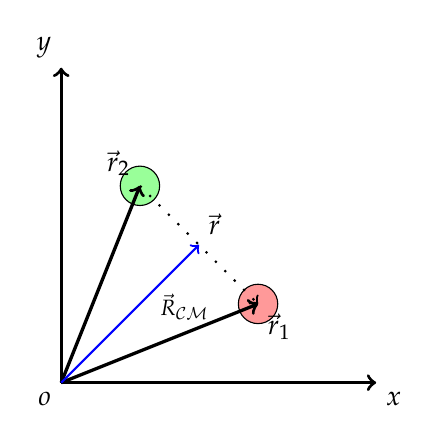
\begin{tikzpicture}
            \coordinate (origin) at (0, 0);
            \coordinate (vec_x) at (4, 0);
            \coordinate (vec_y) at (0, 4);
            \coordinate (vec_r1) at (2.5, 1);
            \coordinate (vec_r2) at (1, 2.5);
            \coordinate (vec_rcm) at (1.75, 1.75);
            
            \node[align = center, anchor = north east] at (origin) {$o$};
            
            \draw[black, very thick, ->](0, 0) -- (vec_x);
            \node[align = center, anchor = north west] at (vec_x) {$x$};
            
            \draw[black, very thick, ->](0, 0) -- (vec_y);
            \node[align = center, anchor = south east] at (vec_y) {$y$};
            
            \filldraw[color = black, fill = red!40](vec_r1) circle (0.25cm);
            \filldraw[color = black, fill = green!40](vec_r2) circle (0.25cm);
            
            \draw[black, very thick, ->](0, 0) -- (vec_r1);
            \node[align = center, anchor = north west] at (vec_r1) {${\vec{r}}_{1}$};
            
            \draw[black, very thick, ->](0, 0) -- (vec_r2);
            \node[align = center, anchor = south east] at (vec_r2) {${\vec{r}}_{2}$};
            
            \draw[black, thick, ->, loosely dotted](vec_r2) -- (vec_r1);
            \node[align = center, anchor = south west] at ($(vec_r2)!0.5!(vec_r1)$) {$\vec{r}$};
            
            \draw[blue, thick, ->](origin) -- (vec_rcm);
            \node[align = center, anchor = north east] at ($(vec_rcm) - (-0.25, 0.5)$) {\footnotesize ${\vec{R}}_{\mathcal{CM}}$};
        \end{tikzpicture}
    \end{figure}
    
    \begin{equation*}
        {\vec{R}}_{\mathcal{CM}} = \frac{{m}_{1} {\vec{r}}_{1} + {m}_{2} {\vec{r}}_{2}}{M}, \qquad M = {m}_{1} + {m}_{2}
    \end{equation*}
    
    et la coordonnée relative entre les deux particules $1$ et $2$ :
    
    \begin{equation*}
        \vec{r} = {\vec{r}}_{1} - {\vec{r}}_{2}, \qquad \frac{1}{\mu} = \frac{1}{{m}_{1}} + \frac{1}{{m}_{2}}
    \end{equation*}
    
    $\mu$ est la masse réduite du système. \\
    
    Par conséquent, on obtient :
    
    \begin{align*}
    \begin{split}
        {\vec{V}}_{\mathcal{CM}} = \frac{{m}_{1} {\vec{v}}_{1} + {m}_{2} {\vec{v}}_{2}}{M} 
            &\iff {\vec{P}}_{\mathcal{CM}} = {\vec{p}}_{1} + {\vec{p}}_{2} \\
        \vec{v} = {\vec{v}}_{1} - {\vec{v}}_{2} 
            &\iff \vec{p} = \frac{{m}_{1} {\vec{p}}_{1} - {m}_{2} {\vec{p}}_{2}}{M}
    \end{split} 
    \end{align*}
    
    \subsection{Hamiltonien classique}
    Dans un référentiel d'inertie, l'énergie mécanique du système de deux particules est :
    
    \begin{equation*}
        {H}_{\mathcal{S}} = \frac{{\vec{p}}_{1}^{2}}{2 {m}_{1}} + \frac{{\vec{p}}_{2}^{2}}{2 {m}_{2}} + V({\vec{r}}_{1} - {\vec{r}}_{2})
    \end{equation*}
    
    En se basant sur les relations donnant les positions ${\vec{R}}_{\mathcal{CM}}$ et $\vec{r}$, on obtient :
    
    \begin{equation*}
    \begin{cases}
        {\vec{r}}_{1} = {\vec{R}}_{\mathcal{CM}} + \frac{{m}_{2}}{M} \vec{r} \\
        {\vec{r}}_{2} = {\vec{R}}_{\mathcal{CM}} - \frac{{m}_{1}}{M} \vec{r}
    \end{cases}
    \end{equation*}
    
    En repportant les expressions de ${\vec{r}}_{1}$ et ${\vec{r}}_{1}$ dans celle de ${H}_{\mathcal{S}}$ et en tenant compte de l'expression de ${\vec{R}}_{\mathcal{CM}}$, on obtient :
    
    \begin{equation*}
    \begin{split}
        {H}_{\mathcal{S}}
            &= \frac{1}{2} M {\vec{V}}_{\mathcal{CM}}^{2} + \frac{1}{2} \mu {\vec{v}}^{2} + V(\vec{r}) \\
            &= \frac{{\vec{P}}_{\mathcal{CM}}^{2}}{2 M} + \frac{{\vec{p}}^{2}}{2 \mu} + V(\vec{r})
    \end{split}
    \end{equation*}
    
    \begin{itemize}
        \itemsep1em
        
        \item 
        Le premier terme représente l'énergie cinétique du centre de masse $\mathcal{CM}$ dans le référentiel d'inertie. Ce terme est nul dans le référentiel de centre de masse.
        
        \item
        Le deuxième terme représente l'énergie du système de deux particules dans le référentiel de centre de masse.
        
        \item
        L'étude du mouvement relatif des deux particules dans le référentiel de CM se mène donc à celle du mouvement de la particule relative de mass $\mu$, de position $\vec{r}$ et d'impulsion $\vec{p}$ plongé dans le potentiel $V(\vec{r})$.
    \end{itemize}
    
    \subsection{Section efficace}
    La modélisation de la collision fait intervenir la notion de \textbf{sections efficace}. Celle-ci est intimement liée à la notion de \textbf{probabilité de diffusion}. \\
    
    Le but de cette modélisation est de pouvoir calculer \textbf{le nombre de collisions qui vont se produire}. \\
    
    Le faisceau incident est caractérisé par sa section transversale de surface $S$. $S$ est la surface de recouvrement (tube de collision) du faisceau sur la cible. Elle est perpendiculaire au faisceau incident. \\
    
   Le module de son courant $\vec{j}$ est donné par $j = D v$, où $v$ est la vitesse moyenne des particules incidentes (projectiles) et $D$ la densité des particules incidentes $n$ par unité de volume $\tau$. \\
    
    Donc :
    
    \begin{equation*}
        j = \frac{n}{\tau} v = \frac{n}{S \Delta l} \frac{\Delta l}{\Delta t} = \frac{n}{S \Delta t}
    \end{equation*}
    
    Ceci permet d'écrire par définition le nombre $n$ de particules traversant la surface $S$ normale au faisceau incident pendant l'intervalle de temps $\diff t$ :
    
    \begin{equation*}
        \diff n = \vec{J} \cdot \vec{\diff S} \, \diff t
    \end{equation*}
    
    \begin{definition}
        $j$ définit le nombre de particules traversant l'unité de surface par unité de temps.
    \end{definition}
    
    Introduisons maintenant le nombre de collisions ${N}_{collision}$ (projectiles-cible) par unité de temps. Ce nombre est propotionnel au courant $j$.
    
    \begin{equation*}
        {N}_{collision} = \sigma j
    \end{equation*}
    
    $\sigma$ est une section efficace.
    
    \begin{definition}
        La section efficace est une grandeur centrale caractérisant la collision entre particules. Physiquement, elle représente le taux ou la probabilité d'une diffusion malgré qu'elle possède les dimensions d'une surface. Elle dépend du potentiel d'interaction entre les deux particules.
    \end{definition}
    
    \section{Déscription quantique d'une collision}
    Les particules incidentes et la cible ont une structure interne :
    
    \begin{itemize}
        \item 
        Particule élémentaire (électron, proton, neutron) : spin
        
        \item
        Particule complexe ou composée (atome, molécule, ion) : nombre quantique $(n, \ l, \ m, \ s)$
    \end{itemize}
    
    \begin{figure}[H]
        \centering
        
        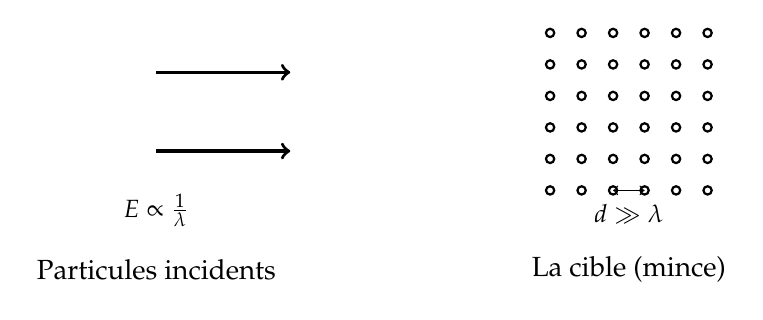
\begin{tikzpicture}
            \coordinate (origin) at (0, 0);
            \coordinate (vec_k) at (1.7, 0);
            
            \draw[black, very thick, ->](-4, 0.5) -- ($(-4, 0.5) + (vec_k)$);
            \draw[black, very thick, ->](-4, -0.5) -- ($(-4, -0.5) + (vec_k)$);
            \node[align = center] at ($(-4, -1.25)$) {\small $E \propto \frac{1}{\lambda}$};
            
            \foreach \x in {0, 1, 2, 3, 4, 5} {
                \foreach \y in {0, 1, 2, 3, 4, 5} {
                    \draw[black, thick]($(origin) + (1 + \x * 0.4, 1 - \y * 0.4)$) circle (1.5pt);
                }
            }
            
            \draw[black, <->]($(origin) + (1.8, -1)$) -- ($(origin) + (2.2, -1)$);
            \node[align = center] at ($(origin) + (2.0, -1.3)$) {\small $d \gg \lambda$};
            
            \node[align = center] at ($(-4, -2)$) {Particules incidents};
            \node[align = center] at ($(2, -2)$) {La cible (mince)};
            
        \end{tikzpicture}
    \end{figure}
    
    Propriétés du faisceau incident :
    
    \begin{itemize}
        \itemsep0.5em
        
        \item
        Monoénergétique.
        
        \item
        Contient du faible nombre de particules (pour ne pas avoir beaucoup  d'interaction entre elles).
    \end{itemize}
    
    \bigskip
    
    Propriétés de la cible :
    
    \begin{itemize}
        \itemsep0.5em
        
        \item 
        Un grande nombre de particules (pour assurer une collision).
        
        \item 
        La distance interne entre les particules de la cible est supérieure à la longeure d'onde du faisceau incident.
        
        \item
        La cible et suffisamment minces pour éviter les diffusion multiples.
    \end{itemize}
    
    \bigskip
    
    Types de collisions :
    
    \begin{itemize}
        \itemsep1.0em
        
        \item 
        Élastique : \ce{A + B -> A + B}, rien n'a changé dans la structure quantique interne des particules (à part leur trajectoire).
        
        \item
        Inélastique : \ce{A + B -> A^{'} + B^{'}}, il y a un changement dans les trajectoires des particules et dans la structure interne (\textbf{e.g.} \ $s = \frac{1}{2}$ devient $s = -\frac{1}{2}$).
        
        \item
        Parfaitement inélastique : \ce{A + B -> C + D}, il y a un changement dans les particules élémentaires : A et B changera en C et D.
    \end{itemize}
    
    \begin{examples}
        \leavevmode
        
        \begin{itemize}
            \item
            \ce{e+ + H -> e+ + H} (diffusion élastique).
            
            \item
            \ce{e+ + H -> e+ + H^{*}} (diffusion inélastique).
            
            \item
            \ce{e+ + H -> e+ + p + e-} (réaction d'ionisation).
            
            \item
            \ce{e+ + H -> p + 2\gamma} (réaction d'annihilation).
            
            \item
            \ce{e+ + H -> p + (e+ + e- )} (réarrangement).
        \end{itemize}
    \end{examples}
    
    Dans tous les cas, l'énergie de la particule incidente est différente.
    
    \subsection{Équation d'onde stationnaire}
    On a un système de deux particules $({m}_{1}, \ {\vec{r}}_{1}, \ {\vec{p}}_{1})$ et $({m}_{2}, \ {\vec{r}}_{2}, \ {\vec{p}}_{2})$, elles interagissent par un potentiel $V({\vec{r}}_{2} - {\vec{r}}_{1})$. \\
    
    L'Hamiltonien du système est donné par :
    
    \begin{equation*}
        {\opr{H}}_{\mathcal{S}} = \frac{{\opr{p}}_{1}^{2}}{2 {m}_{1}} + \frac{{\opr{p}}_{2}^{2}}{2 {m}_{2}} + V({\vec{r}}_{2} - {\vec{r}}_{1})
    \end{equation*}
    
    Donc, on a l'équation de \textsc{Schrödinger} suivante :
    
    \begin{equation*}
        {\opr{H}}_{\mathcal{S}} \Psi({\vec{r}}_{1}, \ {\vec{r}}_{2}, \ t) = \i \hbar \frac{\partial \Psi({\vec{r}}_{1}, \ {\vec{r}}_{2}, \ t)}{\partial t}
    \end{equation*}
    
    Nous avons donc une équation à 7 variables. Le cas au l'Hamiltonien ne dépend pas du temps, on peut faire une séparation de variables.
    
    \begin{equation*}
        \Psi({\vec{r}}_{1}, \ {\vec{r}}_{2}, \ t) = \Phi({\vec{r}}_{1}, \ {\vec{r}}_{2}) f(t)
    \end{equation*}
    
    La condition de normalization $\bigint{}{} \!\! {\left\lvert\Psi({\vec{r}}_{1}, \ {\vec{r}}_{2}, \ t)\right\rvert}^{2} \ {\diff}^{3} {r}_{1} \, {\diff}^{3} {r}_{2} \, \diff t = 1$ implique :
    
    \begin{align*}
    \begin{split}
        \bigint{}{} \!\! {\left\lvert\Phi({\vec{r}}_{1}, \ {\vec{r}}_{2})\right\rvert}^{2} \ {\diff}^{3} {r}_{1} \, {\diff}^{3} {r}_{2} &= 1 \\
        \bigint{}{} \!\! {\left\lvert{f}(t)\right\rvert}^{2} \ \diff t &= 1
    \end{split}
    \end{align*}
    
    Donc $f(t) = {\e}^{\pm \i \omega t}$, avec $\omega = \frac{{E}_{\mathcal{S}}}{\hbar}$. \\
    
    Notre potentiel ne dépend que de ${\vec{r}}_{2} - {\vec{r}}_{1}$, alors ${\opr{H}}_{\mathcal{S}}$ est indépendant du temps, on a donc :
    
    \begin{equation*}
        {\opr{H}}_{\mathcal{S}} \Phi({\vec{r}}_{1}, \ {\vec{r}}_{2}) = {E}_{\mathcal{S}} \Phi({\vec{r}}_{1}, \ {\vec{r}}_{2})
    \end{equation*}
    
    \subsection{Référentiel de centre de masse}
    L'Hamiltonien du système s'écrit :
    
    \begin{equation*}
        {\opr{H}}_{\mathcal{S}} = {\opr{H}}_{\mathcal{CM}} + \opr{H}
    \end{equation*}
    
    avec :
    \begin{align*}
    \begin{split}
        {\opr{H}}_{\mathcal{CM}} &= \frac{{\opr{P}}_{\mathcal{CM}}^{2}}{2 M}, \qquad\qquad M = {m}_{1} + {m}_{2} \\
        \opr{H} &= \frac{{\opr{p}}^{2}}{2 \mu} + V(\vec{r}), \qquad \mu = \frac{{m}_{1} {m}_{2}}{{m}_{1} + {m}_{2}}
    \end{split}
    \end{align*}
    
    L'ensemble $\Big\{{\opr{H}}_{\mathcal{S}}, \ {\opr{H}}_{\mathcal{CM}}, \ \opr{H}\Big\}$ forme un \textbf{ECOC} (ensemble complet d'observables qui commutent). donc il ont un système de vecteurs propres communes. $\Big\{\!\ket{\chi}\!\Big\}$ :
    
    \begin{align*}
    \begin{split}
        {\opr{H}}_{\mathcal{CM}} \ket{\chi} &= {E}_{\mathcal{CM}} \ket{\chi} \\
        \opr{H} \ket{\chi} &= E \ket{\chi} \\
        {\opr{H}}_{\mathcal{S}} \ket{\chi} &= \left({E}_{\mathcal{CM}} + E \right) \ket{\chi}
    \end{split}
    \end{align*}
    
    L'espace d'\textsc{Hilbert} des états est ${\mathcal{H}}_{\mathcal{S}} = {\mathcal{H}}_{\mathcal{CM}} \otimes \mathcal{H}$, et on a comme vecteur $\ket{\Phi} \in {\mathcal{H}}_{\mathcal{S}}$ :
    
    \begin{equation*}
        \ket{\Phi} = \ket{\xi} \otimes \ket{\eta}
    \end{equation*}
    
    avec $\ket{\xi} \in {\mathcal{H}}_{\mathcal{CM}}$ et $\ket{\eta} \in \mathcal{H}$. \\
    
    Si $V(\vec{r})$ dépend de $r = \left\lVert{\vec{r}}_{2} - {\vec{r}}_{1}\right\rVert$ (et non pas de $\vec{r} = {\vec{r}}_{2} - {\vec{r}}_{1})$, le potentiel est dit potentiel central. \\
    
    Donc on a transformé notre problème à un problème de diffusion d'une particule $(\mu, \ \vec{r}, \ \vec{p})$ par un potentiel central $V(r)$.
    
    \subsection{Onde stationnaire de diffusion}
    Soit $E$ l'énergie de la particule relative $(\mu, \ \vec{r}, \ \vec{p})$, $\vec{p} = \hbar \vec{k}$. Quand $V(r) = 0$ :
    
    \begin{equation*}
        E = \frac{{p}^{2}}{2 \mu} = \frac{{\hbar}^{2} {k}^{2}}{2 \mu}
    \end{equation*}
    
    Le faisceau est large, donc le nombre de particules non-diffusées est très grand par rapport au nombre de particules diffusées. Ces particules transmises ne seront pas diffusées par $V(r)$. \\
    
    L'équation de \textsc{Schrödinger} s'écrit sous la forme :
    
    \begin{equation*}
        \left[-\frac{{\hbar}^{2}}{2 \mu} \laplacian + V(r)\right] \Psi(\vec{r}) = E \Psi(\vec{r})
    \end{equation*}
    
    Cette équation admet une infinité de solutions (une pour chaque valeur de $k$). Mais, il faut choisir pour celle-ci, celle qui correspond au problème étudie. \\
    
    Avant d'entrer (selon la direction $oz$) dans la zone d'action de $V(r)$, la particule est considérée comme une onde plane :
    
    \begin{equation*}
        {\Psi}_{inc}(\vec{r}) = {\e}^{\i k z}
    \end{equation*}
    
    Après la diffusion, le paquet d'onde est égale à une partie d'onde transmise, plus une partie d'onde diffusé. On a par définition le comportement asymptotique suivant (pour $r \to \infty$) :
    
    \begin{equation*}
        {\Psi}_{dif}(\vec{r}) = \underbrace{{\e}^{\i k z} \vphantom{f(\theta, \ \phi) \frac{{\e}^{\i k r}}{r}}}_{\text{onde transmise}} + \qquad \underbrace{f(\theta, \ \phi) \frac{{\e}^{\i k r}}{r}}_{\text{onde diffusée}}
    \end{equation*}
    
    Donc, l'onde diffusée dépend de $\vec{r}$ et l'angle solid $\Omega = (\theta, \ \phi)$. $f(\theta, \ \phi)$ est appelée \textbf{amplitude de diffusion}. 
    
    
    
    \chapter{Diffusion par un potentiel central}
    
    \section{Introduction}
    L'analyse d'une collision se fait en décrivant le problème en termes des coordonnées relatives et du centre de masse $\mathcal{CM}$. \\
    
    La dynamique du centre de masse est triviale, et on se concentre sur le mouvement relatif qui est décrit par l'Hamiltonien d'une particule de la masse réduite en interaction avec un potentiel sacré à l'origine. \\
    
    Nous avons déjà fait ça dans le chapitre précédent. Donc, nous allons nous concentrer sur le problème relatif ainsi formulé. \\
    
    La mesure qu'on fait dans une experience de collision, et donc la grandeur qu'on veut calculer est la section efficace différentielle :
    
    \begin{equation*}
        \frac{\diff \sigma(\theta, \ \phi)}{\diff \Omega} = \frac{{j}_{dif}}{{j}_{inc}} {r}^{2}
    \end{equation*}
    
    En tenant compte de l'expression de l'onde diffusée que nous avons déjà calculé :
    
    \begin{equation*}
        {\Psi}_{dif}(\vec{r}) = {\e}^{\i \vec{k} \cdot \vec{r}} + f(\theta, \ \phi) \frac{{\e}^{\i k r}}{r}
    \end{equation*}
    
    On a trouvé :
    
    \begin{equation*}
        \frac{\diff \sigma(\theta, \ \phi)}{\diff \Omega} = {\left\lvert{f}(\theta, \ \phi)\right\rvert}^{2}
    \end{equation*}
    
    Dans ce chapitre on va calculer cette section efficace dans le cas d'une diffusion d'une particule de masse $m$ pour un potentiel central $V(r)$.
    
    \section{Résolution de l'équation de \textsc{Schrödinger} en coordonnées sphériques}
    Pour calculer la section efficace, il faut déterminer la forme asymptotique de l'onde stationnaire $\Psi(\vec{r})$. \\
    
    L'Hamiltonien du système s'écrit :
    
    \begin{equation*}
        \opr{H} = \frac{{\opr{P}}^{2}}{2 m} + V(\vec{r})
    \end{equation*}
    
    $V(\vec{r}) = V(r)$ car le problème présente une symmétrie sphérique. Nous utilisons donc les coordonnées sphériques $(r, \ \theta, \ \phi)$ où :
    
    \begin{equation} \label{ch2eq/1}
    \begin{cases}
        x = r \sin{\theta} \cos{\phi} \\
        y = r \sin{\theta} \sin{\phi} \\
        z = r \cos{\theta}
    \end{cases}
    \end{equation}
    
    Il s'agit de trouver le terme cinétique $\frac{{\opr{P}}^{2}}{2 m} = -\frac{{\hbar}^{2}}{2 m} \laplacian$ où : 
    
    \begin{equation*}
        \laplacian = \frac{{\partial}^{2}}{\partial {x}^{2}} + \frac{{\partial}^{2}}{\partial {y}^{2}} + \frac{{\partial}^{2}}{\partial {z}^{2}}
    \end{equation*}
    
    En utilisant les transformations \eqref{ch2eq/1}, on trouve :
    
    \begin{align*}
    \begin{split}
        \laplacian &= \frac{{\partial}^{2}}{\partial {r}^{2}} + \frac{2}{r} \frac{\partial}{\partial r} - \frac{1}{{\hbar}^{2}} \frac{{\opr{L}}^{2}}{{r}^{2}}, \qquad \vec{L} = \vec{r} \times \vec{p} \\
        {\opr{L}}^{2} &= - {\hbar}^{2} \left(\frac{{\partial}^{2}}{\partial {\theta}^{2}} + \cot{\theta} \frac{\partial}{\partial \theta} + \frac{1}{\sin^2 \theta} \frac{{\partial}^{2}}{\partial {\phi}^{2}}\right)
    \end{split}
    \end{align*}
    
    Donc l'équation de \textsc{Schrödinger} s'écrit :
    
    \begin{equation*}
        \left[-\frac{{\hbar}^{2}}{2 m} \left(\frac{{\partial}^{2}}{\partial {r}^{2}} + \frac{2}{r} \frac{\partial}{\partial r}\right) + \frac{1}{2 m} \frac{{\opr{L}}^{2}}{{r}^{2}} + V(r)\right] \Psi(r, \ \theta, \ \phi) = E \Psi(r, \ \theta, \ \phi)
    \end{equation*}
    
    Selon les expressions de ${\opr{L}}^{2}, \ \opr{H}$ et ${\opr{L}}_{z} = - \i \hbar \frac{\partial}{\partial \phi}$. On déduit que'ils commutent deux à deux. Donc il admettent au minimum un \textbf{ECOC} (ensemble complet d'observables qui commutent). C'est-à-dire, ils partagent un ensemble de fonctions propres communes. \\
    
    On peut trouver cette ensemble parmi les fonctions propres de ${\opr{L}}^{2}$ et ${\opr{L}}_{z}$ que nous connaisons déjà, et qui sont les harmoniques sphériques ${Y}_{l}^{m}(\theta, \ \phi)$. En effet :
    
    \begin{align} \label{ch2eq/2}
    \begin{split}
        {\opr{L}}^{2} {Y}_{l}^{m}(\theta, \ \phi) &= l(l + 1) {\hbar}^{2} {Y}_{l}^{m}(\theta, \ \phi) \\
        {\opr{L}}_{z} {Y}_{l}^{m}(\theta, \ \phi) &= m \hbar {Y}_{l}^{m}(\theta, \ \phi)
    \end{split}
    \end{align}
    
    Donc, nous peuvons écrire les solutions de l'équation de \textsc{Schrödinger} sous la forme :
    
    \begin{equation*}
        \Psi(r, \ \theta, \ \phi) = \sum_{l, m} {R}_{l}(r) {Y}_{l}^{m}(\theta, \ \phi)
    \end{equation*}
    
    \section{Décomposition en onde partielles}
    Comme le faisceau incident ${\vec{k}}_{0}$ est selon la direction $oz$, et le potentiel $V(r)$ est symmétrique, donc $\Psi(r, \ \theta, \ \phi)$ est indépendant de $\phi$, ce qui correspond à $m = 0$ :
    
    \begin{equation*}
        \Psi(r, \ \theta, \ \phi) = \sum_{l} {R}_{l}(r) {Y}_{l}^{0}(\theta, \ \phi)
    \end{equation*}
    
    sachant que ${Y}_{l}^{0}(\theta, \ \phi) \propto {P}_{l}(\cos{\theta})$, on a :
    
    \begin{equation*}
        \Psi(r, \ \theta, \ \phi) = \sum_{l} {R}_{l}(r) {P}_{l}(\cos{\theta})
    \end{equation*}
    
    En autre, en tenant compte de \eqref{ch2eq/2} et en remplaçant dans l'équation de \textsc{Schrödinger}, on trouve :
    
    \begin{equation*}
        \left[-\frac{{\hbar}^{2}}{2 m} \left(\frac{{\partial}^{2}}{\partial {r}^{2}} + \frac{2}{r} \frac{\partial}{\partial r}\right) + \frac{{\hbar}^{2}}{2 m} \frac{l(l + 1)}{{r}^{2}} + V(r) - E\right] {R}_{l}(r) = 0
    \end{equation*}
    
    Nous allons étudier les solutions ${R}_{l}(r)$ pour une valeur positive de l'énergie $E = \frac{{\hbar}^{2}}{2 m} {k}^{2}$. On pose aussi $U(r) = \frac{2 m}{{\hbar}^{2}} V(r)$, On obtient :
    
    \begin{equation*}
        \left[\frac{{\partial}^{2}}{\partial {r}^{2}} + \frac{2}{r} \frac{\partial}{\partial r} - \frac{l(l + 1)}{{r}^{2}} - U(r) + {k}^{2}\right] {R}_{l}(r) = 0
    \end{equation*}
    
    Le but est de chercher le paquet d'onde de l'onde diffusée ${\Psi}_{dif}(\vec{r})$. \\
    
    On sait que loin de $V(r)$, l'onde est stationnaire. Dans la zone d'influence ($V(r) \neq 0$), le paquet d'onde sera perturbé, il prend la forme sphérique. \\
    
    On constate qu'il y a une onde transmise et une onde qui se diffuse dans toutes les directions.
    
    \begin{figure}[H]
        \centering
        
        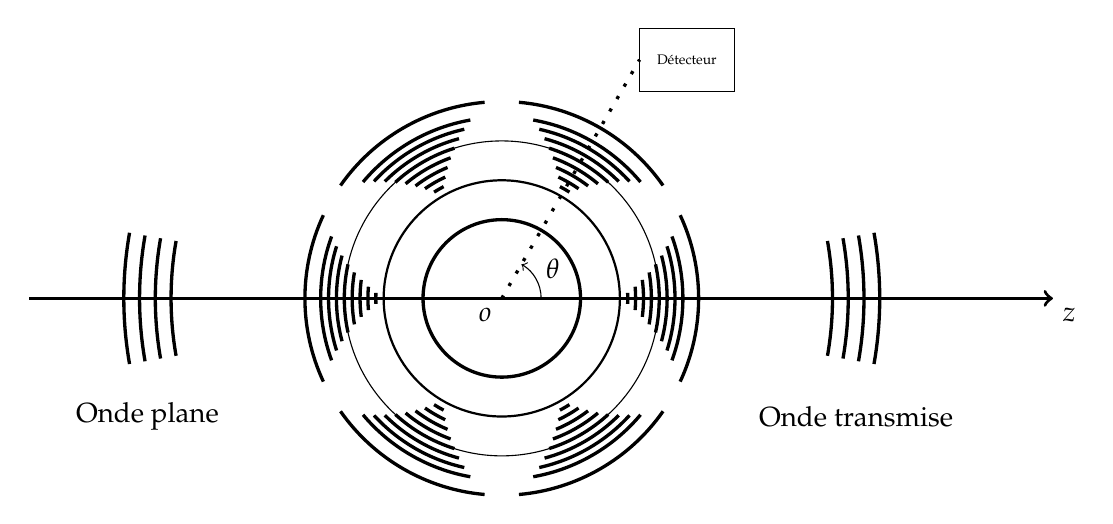
\begin{tikzpicture}
            \coordinate (origin) at (0, 0);
            \coordinate (vec_z) at (7, 0);
            \coordinate (vec_k) at ({3.5 * cos(60)}, {3.5 * sin(60)});
            
            \node[align = center, anchor = north east] at (origin) {$o$};
            
            \draw[black, very thick, ->](-6, 0) -- (vec_z);
            \node[align = center, anchor = north west] at (vec_z) {$z$};
            
            
            \draw[black, very thick, loosely dotted](0, 0) -- (vec_k);

            \draw[black]($(vec_k) - (0, 0.4)$) rectangle ($(vec_k) + (1.2, 0.4)$);
            \node[align = center] at ($(vec_k) + (0.6, 0)$) {\tiny Détecteur};
            
            \draw[black, very thick](origin) circle (1cm);
            \draw[black, thick](origin) circle (1.5cm);
            \draw[black](origin) circle (2cm);
            
            \foreach \y in {1, 2, 3} {
                \foreach \x in {1, 2, 3, 4, 5, 6, 7, 8, 10} {
                    \draw[black, very thick]($(origin) + ({(1.5 + \x * 0.1) * cos(60 * \y - (10 * \x / 4))}, {(1.5 + \x * 0.1) * sin(60 * \y - (10 * \x / 4))})$) arc (60 * \y - 10 * \x / 4:60 * \y + 10 * \x / 4:1.5 + \x * 0.1);
                    \draw[black, very thick]($(origin) - ({(1.5 + \x * 0.1) * cos(60 * \y - (10 * \x / 4))}, {(1.5 + \x * 0.1) * sin(60 * \y - (10 * \x / 4))})$) arc (60 * \y + 180 - 10 * \x / 4:60 * \y + 180 + 10 * \x / 4:1.5 + \x * 0.1);
                }
            }
            
            \foreach \x in {1, 2, 3, 4} {
                \draw[black, very thick]($(origin) + ({(4 + \x * 0.2) * cos(-10)}, {(4 + \x * 0.2) * sin(-10)})$) arc (-10:10:4 + \x * 0.2);
                \draw[black, very thick]($(origin) - ({(4 + \x * 0.2) * cos(-10)}, {(4 + \x * 0.2) * sin(-10)})$) arc (180 - 10:180 + 10:4 + \x * 0.2);
            }
            
            \node[align = center] at ($(origin) - (4.5, 1.5)$) {Onde plane};
            \node[align = center] at ($(origin) + (4.5, -1.5)$) {Onde transmise};
            
            \pic[draw, ->, "$\theta$", angle eccentricity = 1.5] {angle = vec_z--origin--vec_k};
        \end{tikzpicture}
    \end{figure}
    
    Pour une onde stationnaire libre ($V(r) = 0$), l'équation de \textsc{Schrödinger} est sous la forme :
    
    \begin{equation*}
        \left[\laplacian + {k}^{2}\right] \Psi(\vec{r}) = 0
    \end{equation*}
    
    et sa solution est donnée par :
    
    \begin{equation*}
        {\Psi}_{inc}(\vec{r}) = {\e}^{\i \vec{k} \cdot \vec{r}} = {\e}^{\i k z}
    \end{equation*}
    
    L'onde diffusée est ${\Psi}_{dif}(\vec{r}) = {\e}^{\i k z} + \text{onde sphérique}$. \\
    
    A fin d'éviter les interférences entre les 2 ondes (plane et sphérique), on fait nous mesures à $r \to \infty$. Donc en cherche le comportement asymptotique de notre fonction d'onde.
    
    Une onde sphérique a pour forme $\frac{{\e}^{\i k r}}{r}$, le $\frac{1}{r}$ exprime la dispersion de l'onde (diminution de son intensité) en l'assimulant à la lumière, donc :

    \begin{equation*}
        {\Psi}_{asy}(\vec{r}) = {\e}^{\i \vec{k} \cdot \vec{r}} + f(\theta, \ \phi) \frac{{\e}^{\i k r}}{r}
    \end{equation*}
    
    \subsection{Solution de l'équation de \textsc{Schrödinger} asymptotique}
    Lorsque $r \to \infty$, $U(r) = 0$, on obtient l'équation de \textsc{Schrödinger} suivante :
    
    \begin{equation*}
        \left[\frac{{\partial}^{2}}{\partial {r}^{2}} + \frac{2}{r} \frac{\partial}{\partial r} - \frac{l(l + 1)}{{r}^{2}} + {k}^{2}\right] {R}_{l}(r) = 0
    \end{equation*}
    
    En effectant le changement de variable $\rho = k r$, notre équation se ramène à celle de \textsc{Bessel} :
    
    \begin{equation*}
        \left[\frac{{\partial}^{2}}{\partial {\rho}^{2}} + \frac{2}{\rho} \frac{\partial}{\partial \rho} - \frac{l(l + 1)}{{\rho}^{2}} + 1\right] {R}_{l}(\rho) = 0
    \end{equation*}
    
    Les solutions sont données par les fonctions de \textsc{Bessel} sphériques ${Z}_{l}(\rho)$ :
    
    \begin{equation*}
        {Z}_{l}(\rho) = {A}_{l} {J}_{l}(\rho) + {B}_{l} {N}_{l}(\rho)
    \end{equation*}
    
    Donc ${Z}_{l}(\rho)$ est une composition linéaire des fonctions de \textsc{Bessel} ${J}_{l}(\rho)$ et de \textsc{Neumann} ${N}_{l}(\rho)$, dont les comportement asymptotiques sont :
    
    \begin{align*}
    \begin{split}
        \lim_{\rho \to \infty} {J}_{l}(\rho) &\sim \frac{\sin\left(\rho - l \frac{\pi}{2}\right)}{\rho} \\
        \lim_{\rho \to \infty} {N}_{l}(\rho) &\sim -\frac{\cos\left(\rho - l \frac{\pi}{2}\right)}{\rho}
    \end{split}
    \end{align*}
    
    \begin{align*}
    \begin{split}
        \lim_{\rho \to 0} {J}_{l}(\rho) &\sim {\rho}^{l} \\
        \lim_{\rho \to 0} {N}_{l}(\rho) &\sim \frac{1}{{\rho}^{l + 1}}
    \end{split}
    \end{align*}
    
    La solution ${N}_{l}(\rho)$ n'est par régulière, donc nous la rejetterons :
    
    \begin{equation*}
        {R}_{l}(\rho) = {A}_{l} {J}_{l}(\rho) = {A}_{l} \frac{\sin\left(\rho - l \frac{\pi}{2}\right)}{\rho}
    \end{equation*}
    
    ${R}_{l}(\rho)$ représente l'onde plane ($V(r) = 0$), ce qui induit :
    
    \begin{equation*}
        {\Psi}_{inc}(\vec{r}) = {\e}^{\i k z} = \sum_{l} {A}_{l} \frac{\sin\left(k r - l \frac{\pi}{2}\right)}{k r} {P}_{l}(\cos{\theta})
    \end{equation*}
    
    Les ${A}_{l}$ sont des constantes à déterminer. \\
    
    Par conséquent, quand $U(r) \neq 0$, ${R}_{l}(\rho)$ qui représent le paquet d'onde stationnaire diffusé sera influencée par $U(r)$ tel que :
    
    \begin{equation*}
        {R}_{l}^{dif}(r) = {C}_{l} \frac{\sin\left(k r - l \frac{\pi}{2} + {\delta}_{l}\right)}{k r}
    \end{equation*}
    
    ${\delta}_{l}$ est le déphasage apporté par le potentiel $V(r)$ (ou $U(r)$). Par conséquent, le paquet d'onde totale prend la forme suivante :
    
    \begin{equation*}
        {\Psi}_{dif}(r, \ \theta, \ \phi) = \sum_{l} {C}_{l} \frac{\sin\left(k r - l \frac{\pi}{2} + {\delta}_{l}\right)}{k r} {P}_{l}(\cos{\theta})
    \end{equation*}
    
    \section{Calcul de l'amplitude de diffusion}
    Afin de calculer l'amplitude de diffusion $f(\theta, \ \phi)$, on est amené à comparer entre le paquet d'onde en présence de $V(r)$ à savoir : 
    
    \begin{equation} \label{ch2eq/3}
        {\Psi}_{dif}(r, \ \theta, \ \phi) = \sum_{l} {C}_{l} \frac{\sin\left(k r - l \frac{\pi}{2} + {\delta}_{l}\right)}{k r} {P}_{l}(\cos{\theta})
    \end{equation}
    
    et la fonction d'onde asymptotique :
    \begin{equation} \label{ch2eq/4}
        {\Psi}_{asy}(\vec{r}) = {\e}^{\i \vec{k} \cdot \vec{r}} + f(\theta, \ \phi) \frac{{\e}^{\i k r}}{r}
    \end{equation}
    
    Donc, il est nécessaire de développer l'onde plane en polynômes de \textsc{Legendre}. \\
    
    En effet, selon la solution de l'équation de \textsc{Schrödinger} quand $V(r) = 0$, on a trouvé :
    
    \begin{equation*}
        {R}_{l}(r) = {A}_{l} \frac{\sin\left(k r - l \frac{\pi}{2}\right)}{k r}
    \end{equation*}
    
    avec \footnote{Voir le livre "Quantum Mechanics" par \textsc{Albert Messiah}} ${A}_{l} = {i}^{l} (2l + 1)$.
    
    \begin{equation*}
        {\Psi}_{inc}(\vec{r}) = {\e}^{\i k z} = \sum_{l} {i}^{l} (2l + 1) \frac{\sin\left(k r - l \frac{\pi}{2}\right)}{k r} {P}_{l}(\cos{\theta})
    \end{equation*}
    
    En autre, $f(\theta, \ \phi)$ est aussi développé en polynômes de \textsc{Legendre}.
    
    \begin{equation*}
        f(\theta, \ \phi) = \sum_{l} {f}_{l} {P}_{l}(\cos{\theta})
    \end{equation*}
    
    L'équation \eqref{ch2eq/4} devient:

    \begin{equation} \label{ch2eq/5}
        {\Psi}_{asy}(r, \ \theta, \ \phi) = \sum_{l} \left[{i}^{l} (2l + 1) \frac{\sin\left(k r - l \frac{\pi}{2}\right)}{k r} + {f}_{l} \frac{{\e}^{\i k r}}{r}\right] {P}_{l}(\cos{\theta})
    \end{equation}
    
    Développons le $\sin$ dans l'équatiion \eqref{ch2eq/3} :
    \begin{equation*}
        {\Psi}_{dif}(r, \ \theta, \ \phi) = \sum_{l} {C}_{l} \frac{\sin\left(k r - l \frac{\pi}{2}\right) \cos{{\delta}_{l}} + \cos\left(k r - l \frac{\pi}{2}\right) \sin{{\delta}_{l}}}{k r} {P}_{l}(\cos{\theta})
    \end{equation*}
    
    Selon \textsc{Euler} :
    
    \begin{equation*}
    \begin{split}
        \cos\left(k r - l \frac{\pi}{2}\right) 
            &= {\e}^{\i \left(k r - l \frac{\pi}{2}\right)} - \i \sin\left(k r - l \frac{\pi}{2}\right) \\
            &= {\left({\e}^{-\i \frac{\pi}{2}}\right)}^{l} {\e}^{\i k r} - \i \sin\left(k r - l \frac{\pi}{2}\right) \\
            &= {(-\i)}^{l} {\e}^{\i k r} - \i \sin\left(k r - l \frac{\pi}{2}\right)
    \end{split}
    \end{equation*}
    
    D'où :
    \begin{equation*}
    \begin{split}
        \sin\left(k r - l \frac{\pi}{2} + {\delta}_{l}\right) 
            &= \sin\left(k r - l \frac{\pi}{2}\right) \cos{{\delta}_{l}} + \cos\left(k r - l \frac{\pi}{2}\right) \sin{{\delta}_{l}} \\
            &= \sin\left(k r - l \frac{\pi}{2}\right) \cos{{\delta}_{l}} + {(-\i)}^{l} {\e}^{\i k r} \sin{{\delta}_{l}} - \i \sin\left(k r - l \frac{\pi}{2}\right) \sin{{\delta}_{l}} \\
            &= \sin\left(k r - l \frac{\pi}{2}\right) \left(\cos{{\delta}_{l}} - \i \sin{{\delta}_{l}}\right) + {(-\i)}^{l} {\e}^{\i k r} \sin{{\delta}_{l}} \\
            &= \sin\left(k r - l \frac{\pi}{2}\right) {\e}^{-\i {\delta}_{l}} + {(-\i)}^{l} {\e}^{\i k r} \sin{{\delta}_{l}}
    \end{split}
    \end{equation*}
    
    Ce qui donne :

    \begin{equation*}
        {\Psi}_{dif}(r, \ \theta, \ \phi) = \sum_{l} {C}_{l} \left[{\e}^{-\i {\delta}_{l}} \frac{\sin\left(k r - l \frac{\pi}{2}\right)}{k r} + {(-\i)}^{l} \frac{\sin{{\delta}_{l}}}{k} \frac{{\e}^{\i k r}}{r}\right] {P}_{l}(\cos{\theta})
    \end{equation*}

    Sa comparaison avec l'équation \eqref{ch2eq/5} donne :
    
    \begin{align*}
    \begin{split}
        {C}_{l} &= {i}^{l} (2l + 1) {\e}^{\i {\delta}_{l}} \\
        {f}_{l} &= {(-\i)}^{l} {C}_{l} \frac{\sin{{\delta}_{l}}}{k} = (2l + 1) \frac{\sin{{\delta}_{l}}}{k} {\e}^{\i {\delta}_{l}}
    \end{split}
    \end{align*}
    
    Par conséquent, l'amplitude de diffusion sera donnée par cette expression :
    
    \begin{equation} \label{ch2eq/6}
        f(\theta, \ \phi) = \frac{1}{k} \sum_{l} (2l + 1) \sin{{\delta}_{l}} {\e}^{\i {\delta}_{l}} {P}_{l}(\cos{\theta})
    \end{equation}
    
    \subsection{Calcul de la section efficace}
    On a :
    
    \begin{equation*}
    \begin{split}
        \frac{\diff \sigma(\theta, \ \phi)}{\diff \Omega} 
            &= {\left\lvert{f}(\theta, \ \phi)\right\rvert}^{2} \\
            &= \frac{1}{{k}^{2}} \sum_{l, m} (2l + 1)(2m + 1) \sin{{\delta}_{l}} \sin{{\delta}_{m}} {\e}^{\i \left({\delta}_{l} - {\delta}_{m}\right)} {P}_{l}(\cos{\theta}) {P}_{m}(\cos{\theta})
    \end{split}
    \end{equation*}
    
    Et on intégrant sur l'angle solide, on obtient \footnote{On a utilié le fait que : 
        \begin{equation*}
            \int_{-1}^{1} \!\!\! {P}_{l}(\cos{\theta}) {P}_{m}(\cos{\theta}) \ \diff \cos{\theta} = \frac{2}{2l + 1} {\delta}_{l, m}
        \end{equation*}}:
    \begin{equation*}
    \begin{split}
        \sigma(\theta, \ \phi)
            &= \iint \frac{\diff \sigma(\theta, \ \phi)}{\diff \Omega} \sin{\theta} \ \diff \theta \ \diff \phi \\
            &= \frac{1}{{k}^{2}} \sum_{l, m} (2l + 1)(2m + 1) \sin{{\delta}_{l}} \sin{{\delta}_{m}} {\e}^{\i \left({\delta}_{l} - {\delta}_{m}\right)} \int_{0}^{\pi} \!\!\! {P}_{l}(\cos{\theta}) {P}_{m}(\cos{\theta}) \sin{\theta} \ \diff \theta \int_{0}^{2\pi} \!\!\!\! \diff \phi \\
            &= \frac{2\pi}{{k}^{2}} \sum_{l, m} (2l + 1)(2m + 1) \sin{{\delta}_{l}} \sin{{\delta}_{m}} {\e}^{\i \left({\delta}_{l} - {\delta}_{m}\right)} \int_{-1}^{1} \!\!\! {P}_{l}(\cos{\theta}) {P}_{m}(\cos{\theta}) \ \diff \cos{\theta} \\
            &= \frac{4\pi}{{k}^{2}} \sum_{l} (2l + 1) \sin^2 {{\delta}_{l}}
    \end{split}
    \end{equation*}
    
    \section{Le sens physique du déphasage}
    Quel est le sense physique du déphasage ${\delta}_{l}$? afin de répondre à cette question, on compare entre l'onde libre (plane) et l'onde diffusée :
    
    \begin{equation*}
        {\Psi}_{inc}(r, \ \theta, \ \phi) = \sum_{l} {R}_{l}^{inc}(r) {P}_{l}(\cos{\theta})
    \end{equation*}
    et
    \begin{equation*}
        {\Psi}_{dif}(r, \ \theta, \ \phi) = \sum_{l} {R}_{l}^{dif}(r) {P}_{l}(\cos{\theta})
    \end{equation*}
    
    On a :

    
    \begin{equation} \label{ch2eq/7}
    \begin{split}
        {R}_{l}^{inc}(r) 
            &= {A}_{l} \frac{\sin\left(k r - l \frac{\pi}{2}\right)}{k r} \\
            &= \frac{{A}_{l}}{2 \i k r} \left[{\e}^{\i \left(k r - l \frac{\pi}{2}\right)} - {\e}^{-\i \left(k r - l \frac{\pi}{2}\right)}\right] \\
            &= \frac{{i}^{l} (2l + 1)}{2 \i k r} \left[{(-\i)}^{l} {\e}^{\i k r} - {\i}^{l} {\e}^{-\i k r}\right] \\
            &= \frac{2l + 1}{2 \i k r} \left[{(-1)}^{l + 1} \underbrace{{\e}^{-\i k r}}_{\text{onde entrante}} + \underbrace{{\e}^{\i k r}}_{\text{onde sortante}}\right]
    \end{split}
    \end{equation}
    
    \begin{remark}
        Ici, il est important de ne pas interpréter l'onde sortante comme une onde diffusée, car il n'y a pas de diffusion dans ${\Psi}_{inc}(\vec{r})$.
    \end{remark}
    
    \begin{equation} \label{ch2eq/8}
    \begin{split}
        {R}_{l}^{dif}(r) 
            &= {C}_{l} \frac{\sin\left(k r - l \frac{\pi}{2} + {\delta}_{l}\right)}{k r} \\
            &= {C}_{l} \frac{\sin\left(k r - l \frac{\pi}{2}\right) {\e}^{-\i {\delta}_{l}} + {(-\i)}^{l} {\e}^{\i k r} \sin{{\delta}_{l}}}{k r} \\
            &= {C}_{l} \frac{\left[{\e}^{\i \left(k r - l \frac{\pi}{2}\right)} - {\e}^{-\i \left(k r - l \frac{\pi}{2}\right)}\right] {\e}^{-\i {\delta}_{l}} + {(-\i)}^{l} {\e}^{\i k r} \left[{\e}^{\i {\delta}_{l}} - {\e}^{-\i {\delta}_{l}}\vphantom{{\e}^{\i \left(k r - l \frac{\pi}{2}\right)}}\right]}{2 \i k r} \\
            &= \frac{{i}^{l} (2l + 1) {\e}^{\i {\delta}_{l}}}{2 \i k r} \Bigg\{\!\!\!\left[{(-\i)}^{l} {\e}^{\i k r} - {\i}^{l} {\e}^{-\i k r}\right] {\e}^{-\i {\delta}_{l}} + {(-\i)}^{l} {\e}^{\i k r} \left[{\e}^{\i {\delta}_{l}} - {\e}^{-\i {\delta}_{l}}\vphantom{{(-\i)}^{l} {\e}^{\i k r}}\right]\!\!\!\Bigg\} \\
            &= \frac{(2l + 1)}{2 \i k r} \left[{(-1)}^{l + 1} \underbrace{{\e}^{-\i k r}}_{\text{onde entrante}} + \ {\e}^{2\i {\delta}_{l}} \underbrace{{\e}^{\i k r}}_{\text{onde sortante}}\right] \\
    \end{split}
    \end{equation}
    
    La comparaison entre \eqref{ch2eq/7} et \eqref{ch2eq/8} montre que l'onde entrante reste la même, tandis que l'onde sortante change de comportement. \\
    
    Donc, le rôle de $V(r)$ est d'introduire un déphasage dans l'onde sortante. \\
    
    On a alors :
    \begin{align*}
    \begin{split}
        {\Psi}_{dif}(r, \ \theta, \ \phi) &= \sum_{l} \frac{(2l + 1)}{2 \i k r} \left[{(-1)}^{l + 1} {\e}^{-\i k r} + {\e}^{2\i {\delta}_{l}} {\e}^{\i k r}\right] {P}_{l}(\cos{\theta}) \\
        {\Psi}_{asy}(r, \ \theta, \ \phi) &= \sum_{l} \frac{(2l + 1)}{2 \i k r} \left[{(-1)}^{l + 1} {\e}^{-\i k r} + {\e}^{\i k r}\right] {P}_{l}(\cos{\theta}) \\
    \end{split}
    \end{align*}
    
    Sous l'effet du potentiel, si on pose \footnote{${S}_{l}(k)$ est appelé l'élément de la matrice $\mathbb{S}$.} ${S}_{l}(k) = {\e}^{2\i {\delta}_{l}(k)}$, on obtient :
    
    \begin{equation*}
        {\Psi}_{dif}(r, \ \theta, \ \phi) = \sum_{l} \frac{(2l + 1)}{2 \i k r} \left[{(-1)}^{l + 1} {\e}^{-\i k r} + {S}_{l}(k) {\e}^{\i k r}\right] {P}_{l}(\cos{\theta})
    \end{equation*}
    
    \bigskip
    
    Equivalement, on peut écrire :
    \begin{equation*}
    \begin{split}
        {\Psi}_{dif}(r, \ \theta, \ \phi) 
            &= {\e}^{\i k z} - {\e}^{\i k z} + \sum_{l} \frac{(2l + 1)}{2 \i k r} \left[{(-1)}^{l + 1} {\e}^{-\i k r} + {S}_{l}(k) {\e}^{\i k r}\right] {P}_{l}(\cos{\theta}) \\
            &= {\e}^{\i k z} - {\Psi}_{asy}(r, \ \theta, \ \phi) + \sum_{l} \frac{(2l + 1)}{2 \i k r} \left[{(-1)}^{l + 1} {\e}^{-\i k r} + {S}_{l}(k) {\e}^{\i k r}\right] {P}_{l}(\cos{\theta}) \\
            &= {\e}^{\i k z} + \sum_{l} \frac{(2l + 1)}{2 \i k} \left({S}_{l}(k) - 1\right) {P}_{l}(\cos{\theta}) \frac{{\e}^{\i k r}}{r}
    \end{split}
    \end{equation*}
    
    Ce qui induit :
    \begin{equation*}
        f(\theta, \ \phi) = \frac{1}{2 \i k} \sum_{l} (2l + 1) \left({S}_{l}(k) - 1\right) {P}_{l}(\cos{\theta})
    \end{equation*}
    
    qui est équivalent à \eqref{ch2eq/6}. \\
    
    Si $\theta = 0 \implies {P}_{l}(\cos{\theta}) = {P}_{l}(1) = 1$, on a :
    
    \begin{equation*}
        f(0, \ \phi) = \frac{1}{k} \sum_{l} (2l + 1) \sin{{\delta}_{l}} {\e}^{\i {\delta}_{l}}
    \end{equation*}
    
    Donc : 
    
    \begin{equation*}
        \sigma(0, \ \phi) = \frac{4\pi}{{k}^{2}} \sum_{l} (2l + 1) \sin^2 {{\delta}_{l}} = \frac{4\pi}{k} \Im f(0, \ \phi)
    \end{equation*}
    
    Ce résultat est connu par le \textbf{théorème optique}.
    
    
    
    \chapter{Fonction de \textsc{Green} - Approximation de \textsc{Born}}
    
    \section{Équation intégrale de diffusion}
    Pour des commodités de calcul, nous allons adopter dans ce qui va suivre, les notations de l'algèbre de \textsc{Dirac}. \\
    
    Soit la diffusion élastique d'une particule de masse $m$ par un potentiel $\mathrm{{V}}(\vec{{r}})$. \\
    
    Soient ${\opr{H}}_{0}$ l'Hamiltonien de la particule incident et $\ket{{\vec{k}}_{0}}$ les kets propres de ${\opr{H}}_{0}$.
    
    \begin{equation*}
        {\opr{H}}_{0} \ket{{\vec{k}}_{0}} = {E}_{0} \ket{{\vec{k}}_{0}}
    \end{equation*}
    
    $\ket{{\vec{k}}_{0}}$ représente l'onde plane incidente ou les particules transmissent sans diffusion.
    
    \begin{equation*}
        \opr{H} = {\opr{H}}_{0} + \opr{V} \implies \opr{V} = \opr{H} - {\opr{H}}_{0}
    \end{equation*}
    
    Après diffusion :
    
    \begin{equation*}
        \opr{H} \ket{{\Psi}_{{\vec{k}}_{f}}} = E \ket{{\Psi}_{{\vec{k}}_{f}}}
    \end{equation*}
    
    $\ket{{\Psi}_{{\vec{k}}_{f}}}$ est associé à la fonction d'onde diffusée qui a le comportement asymptotique suivant :
    
    \begin{equation} \label{chap3_eq/3}
        \ket{{\Psi}_{{\vec{k}}_{f}}} = \ket{{\vec{k}}_{0} \vphantom{{\Psi}_{{\vec{k}}_{f}}}} + \ket{\chi \vphantom{{\Psi}_{{\vec{k}}_{f}}}}
    \end{equation}
    
    où $\ket{\chi}$ représente la partie purement diffusée. On a une diffusion élastique, alors $E = {E}_{0}$ et donc $\ket{{\vec{k}}_{f}} = \ket{{\vec{k}}_{0}}, \ \left\lVert {\vec{k}}_{f} \right\rVert = \left\lVert {\vec{k}}_{0} \right\rVert$. \\
    
    L'action de $\opr{V} \ket{{\Psi}_{{\vec{k}}_{f}}}$ : 
    
    \begin{equation*}
    \begin{split}
        \opr{V} \ket{{\Psi}_{{\vec{k}}_{f}}} 
            &= \left(\opr{H} - {\opr{H}}_{0}\right) \ket{{\Psi}_{{\vec{k}}_{f}}} \\
            &= \left(E - {\opr{H}}_{0}\right) \ket{{\Psi}_{{\vec{k}}_{f}}} \\
            &= \left({E}_{0} - {\opr{H}}_{0}\right) \left(\ket{{\vec{k}}_{0}} + \ket{\chi \vphantom{{\vec{k}}_{0}}}\right) \\
            &= \left({E}_{0} - {\opr{H}}_{0}\right) \ket{{\vec{k}}_{0}} + \left(E - {\opr{H}}_{0}\right) \ket{\chi \vphantom{{\vec{k}}_{0}}} \\
            &= \left({E}_{0} - {\opr{H}}_{0}\right) \ket{\chi \vphantom{{\vec{k}}_{0}}}
    \end{split}
    \end{equation*}
    
    C'est une équation différentielle du second ordre. \\
    
    Si l'on suppose que $\left({E}_{0} - {\opr{H}}_{0}\right)$ est inversible, on a :
    
    \begin{equation} \label{chap3_eq/5}
        \ket{\chi \vphantom{{\Psi}_{{\vec{k}}_{f}}}} = \frac{1}{{E}_{0} - {\opr{H}}_{0}} \opr{V} \ket{{\Psi}_{{\vec{k}}_{f}}}
    \end{equation}
    
    et on appelle opérateur de \textsc{Green} le rapport :
    
    \begin{equation*}
        \opr{G}_{0}({E}_{0}) = \frac{1}{{E}_{0} - {\opr{H}}_{0}}
    \end{equation*}
    
    avec ${E}_{0} > 0$ : la particule incidente avec une énergie cinétique positive et elle est libre. \\
    
    Donc l'équation \eqref{chap3_eq/5} s'écrit :
    
    \begin{equation*}
        \ket{\chi \vphantom{{\Psi}_{{\vec{k}}_{f}}}} = \opr{G}_{0}({E}_{0}) \opr{V} \ket{{\Psi}_{{\vec{k}}_{f}}}
    \end{equation*}
    
    et en remplaçant dans l'équation \eqref{chap3_eq/3}, on a :
    
    \begin{equation*}
        \ket{{\Psi}_{{\vec{k}}_{f}}} = \ket{{\vec{k}}_{0} \vphantom{{\Psi}_{{\vec{k}}_{f}}}} + \opr{G}_{0}({E}_{0}) \opr{V} \ket{{\Psi}_{{\vec{k}}_{f}}}
    \end{equation*}
    
    C'est l'équation intégrale de diffusion en notation de \textsc{Dirac}. \\
    
    Multiplions cette expression par le bra $\bra{\vec{r}}$ (projection dans l'espace des vecteurs positions).
    
    \begin{equation*}
    \begin{split}
        \bra{\vec{r}} \ket{{\Psi}_{{\vec{k}}_{f}}} 
            &= \bra{\vec{r}} \ket{{\vec{k}}_{0}} + \bra{\vec{r} \vphantom{{\Psi}_{{\vec{k}}_{f}}}} \opr{G}_{0}({E}_{0}) \opr{\identity} \opr{V} \ket{{\Psi}_{{\vec{k}}_{f}}} \\
            &= \bra{\vec{r}} \ket{{\vec{k}}_{0}} + \iint \bra{\vec{r} \vphantom{\pvec{r}'}} \opr{G}_{0}({E}_{0}) \ket{\pvec{r}'} \bra{\pvec{r}'} \opr{V} \ket{\pvec{r}''} \bra{\pvec{r}''} \ket{{\Psi}_{{\vec{k}}_{f}}} \ {\diff}^{3} r' \, {\diff}^{3} r''
    \end{split}
    \end{equation*}
    
    On sait que :
    
    \begin{align*}
    \begin{split}
        \bra{\vec{r}} \ket{{\Psi}_{{\vec{k}}_{f}}} &= {\Psi}_{{\vec{k}}_{f}}(\vec{r}) \\
        \bra{\vec{r}} \ket{{\vec{k}}_{0}} &= \frac{{\e}^{\i {\vec{k}}_{0} \cdot \vec{r}}}{(2\pi)^{\frac{3}{2}}}
    \end{split}
    \end{align*}
    
    On notera :
    
    \begin{align*}
    \begin{split}
        \bra{\vec{r} \vphantom{\pvec{r}'}} \opr{G}_{0}({E}_{0}) \ket{\pvec{r}'} &= {G}_{0}(\vec{r}, \ \pvec{r}'; \ {E}_{0}) \\
        \bra{\pvec{r}'} \opr{V} \ket{\pvec{r}''} &= V(\pvec{r}', \ \pvec{r}'')
    \end{split}
    \end{align*}
    
    On a alors :
    
    \begin{equation} \label{chap3_eq/11}
        {\Psi}_{{\vec{k}}_{f}}(\vec{r}) = \frac{{\e}^{\i {\vec{k}}_{0} \cdot \vec{r}}}{(2\pi)^{\frac{3}{2}}} + \iint {G}_{0}(\vec{r}, \ \pvec{r}'; \ {E}_{0}) V(\pvec{r}', \ \pvec{r}'') {\Psi}_{{\vec{k}}_{f}}(\pvec{r}'') \ {\diff}^{3} r' \, {\diff}^{3} r''
    \end{equation}
    
    \bigskip
    
    \begin{itemize}
        \itemsep0.5em
        
        \item
        ${\opr{V}}^{\dagger} = \opr{V}$ potentiel réel $\implies \bra{\pvec{r}'} \opr{V} \ket{\pvec{r}''} = \bra{\pvec{r}''} \opr{V} \ket{\pvec{r}'}$, \\ $V(\pvec{r}', \ \pvec{r}'') = V(\pvec{r}'', \ \vec{r'})$ potentiel symétrique en $\pvec{r}'$ et $\pvec{r}''$.
        
        \item
        Potentiel séparable : $V(\pvec{r}', \ \pvec{r}'') = v(\pvec{r}') v(\pvec{r}'')$ (la même fonction car $V$ est symétrique).
        
        \item
        Un potentiel local est defini par : $V(\pvec{r}', \ \pvec{r}'') = V(\pvec{r}') \delta(\pvec{r}' - \pvec{r}'')$
    \end{itemize}
    
    \section{Fonction de \textsc{Green}}
    On appelle fonction de \textsc{Green} de diffusion ${G}_{0}(\vec{r}, \ \pvec{r}'; \ {E}_{0})$ l'élement de la matrice $\bra{\vec{r}} \opr{G}_{0}({E}_{0}) \ket{\pvec{r}'}$ de l'opérateur de \textsc{Green} $\opr{G}_{0}({E}_{0})$.
    
    \subsection{Calcul de \texorpdfstring{${G}_{0}(\vec{r}, \ \pvec{r}'; \ {E}_{0})$}{G}}
    
    \begin{equation*}
        \opr{G}_{0}({E}_{0}) = \frac{1 \times \opr{\identity}}{{E}_{0} - {\opr{H}}_{0}}, \qquad \opr{\identity} = \bigint{}{} \ket{\vec{k}} \bra{\vec{k}} \ {\diff}^{3} k
    \end{equation*}
    
    Où $\ket{\vec{k}}$ est un ket propre de ${\opr{H}}_{0}$
    
    \begin{equation*}
        {\opr{H}}_{0} \ket{\vec{k}} = E \ket{\vec{k}} = \frac{{\hbar}^{2} {k}^{2}}{2m} \ket{\vec{k}}
    \end{equation*}
    
    \begin{equation*}
        \opr{G}_{0}({E}_{0}) = \Bigint{}{} \frac{\ket{\vec{k}} \bra{\vec{k}}}{{E}_{0} - {E}_{k}} \ {\diff}^{3} k = \frac{2m}{{\hbar}^{2}} \Bigint{}{} \frac{\ket{\vec{k}} \bra{\vec{k}}}{{k}_{0}^{2} - {k}^{2}} \ {\diff}^{3} k
    \end{equation*}
    
    \begin{equation*}
    \begin{split}
        {G}_{0}(\vec{r}, \ \pvec{r}'; \ {E}_{0}) 
            &= \frac{2m}{{\hbar}^{2}} \Bigint{}{} \frac{\bra{\vec{r}} \ket{\vec{k}} \bra{\vec{k}} \ket{\pvec{r}'}}{{k}_{0}^{2} - {k}^{2}} \ {\diff}^{3} k \\
            &= \frac{2m}{{\hbar}^{2}} \frac{1}{{(2\pi)}^{3}} \Bigint{}{} \frac{{\e}^{\i \vec{k} \cdot \vec{r}} \, {\e}^{-\i \vec{k} \cdot \pvec{r}'}}{{k}_{0}^{2} - {k}^{2}} \ {\diff}^{3} k \\
            &= \frac{2m}{{\hbar}^{2}} \frac{1}{{(2\pi)}^{3}} \Bigint{}{} \frac{{\e}^{\i \vec{k} \cdot \left(\vec{r} - \pvec{r}'\right)}}{{k}_{0}^{2} - {k}^{2}} \ {\diff}^{3} k
    \end{split}
    \end{equation*}
    
    On montre que ${G}_{0}(\vec{r}, \ \pvec{r}'; \ {E}_{0}) = {G}_{0}(\vec{r} - \pvec{r}'; \ {E}_{0})$ n'est qu'une fonction de $\vec{r} - \pvec{r}'$. \\
    
    On pose $\vec{\rho} = \vec{r} - \pvec{r}'$ et choisissons $\vec{\rho}$ le long de l'axe $oz$ et on utilise les coordonnées sphériques :
    
    \begin{figure}[H]
        \centering
        
        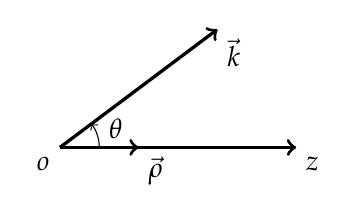
\begin{tikzpicture}
            \coordinate (origin) at (0, 0);
            \coordinate (vec_z) at (3, 0);
            \coordinate (vec_rho) at (1, 0);
            \coordinate (vec_k) at (2, 1.5);
            
            \node[align = center, anchor = north east] at (origin) {$o$};
            
            \draw[black, very thick, ->](0, 0) -- (vec_z);
            \node[align = center, anchor = north west] at (vec_z) {$z$};
            
            \draw[black, very thick, ->](0, 0) -- (vec_rho);
            \node[align = center, anchor = north west] at (vec_rho) {$\vec{\rho}$};
            
            \draw[black, very thick, ->](0, 0) -- (vec_k);
            \node[align = center, anchor = north west] at (vec_k) {$\vec{k}$};
            
            \pic[draw, ->, "$\theta$", angle eccentricity = 1.5] {angle = vec_rho--origin--vec_k};
        \end{tikzpicture}
    \end{figure}
    
    \begin{align*}
    \begin{split}
        \vec{k} \cdot \left(\vec{r} - \pvec{r}'\right) &= \vec{k} \cdot \vec{\rho} = k \rho \cos{\theta} \\
        {\diff}^{3} k &= {k}^{2} \sin{\theta} \ \diff k \, \diff \theta \, \diff \phi
    \end{split}
    \end{align*}
    
    \begin{equation*}
        {G}_{0}(\rho; \ {E}_{0}) = \frac{2m}{{\hbar}^{2}} \frac{1}{{(2\pi)}^{3}} \Bigint{0}{\infty} \removeintspace \ \frac{{k}^{2}}{{k}_{0}^{2} - {k}^{2}} \ \diff k \ \Bigint{0}{2\pi} \removeintspace \diff \phi \ \Bigint{0}{\pi} \removeintspace {\e}^{\i k \rho \cos{\theta}} \sin{\theta} \ \diff \theta
    \end{equation*}
    
    Posons $u = \cos{\theta}, \ du = - \sin{\theta} \ \diff \theta$
    
    \begin{equation*}
    \begin{split}
        \Bigint{0}{\pi} \removeintspace {\e}^{\i k \rho \cos{\theta}} \sin{\theta} \ \diff \theta 
            &= \int_{-1}^{1} {\e}^{\i k \rho u} \ \diff u \\
            &= \frac{1}{\i k \rho} \left[{\e}^{\i k \rho u}\right]_{-1}^{+1} \\
            &= \frac{1}{\i k \rho} \left[{\e}^{\i k \rho} - {\e}^{-\i k \rho}\right] \\
            &= \frac{2}{k \rho} \left[\frac{{\e}^{\i k \rho} - {\e}^{-\i k \rho}}{2 \i}\right]
    \end{split}
    \end{equation*}
    
    \begin{equation*}
        \Bigint{0}{\pi} \removeintspace {\e}^{\i k \rho \cos{\theta}} \sin{\theta} \ \diff \theta = 2 \frac{\sin{k \rho}}{k \rho}
    \end{equation*}
    
    On a alors :
    
    \begin{equation*}
    \begin{split}
        {G}_{0}(\rho; \ {E}_{0}) 
            &= \frac{2m}{{\hbar}^{2}} \frac{1}{{(2\pi)}^{3}} \frac{4\pi}{\rho} \Bigint{0}{\infty} \removeintspace \ \underbrace{\frac{k \sin{k \rho}}{{k}_{0}^{2} - {k}^{2}}}_{\text{pair}} \ \diff k \\
            &= \frac{2m}{{\hbar}^{2}} \frac{1}{{(2\pi)}^{3}} \frac{4\pi}{\rho} \frac{1}{2} \Bigint{-\infty}{+\infty} \removeintspace \ \frac{k \sin{k \rho}}{{k}_{0}^{2} - {k}^{2}} \ \diff k \\
            &= \frac{m}{2 \rho {\pi}^{2} {\hbar}^{2}} \Bigint{-\infty}{+\infty} \removeintspace \ \frac{k \sin{k \rho}}{{k}_{0}^{2} - {k}^{2}} \ \diff k \\
            &= \frac{m}{2 \rho {\pi}^{2} {\hbar}^{2}} \ \Im \!\!\! \Bigint{-\infty}{+\infty} \removeintspace \ \frac{k {\e}^{\i k \rho}}{{k}_{0}^{2} - {k}^{2}} \ \diff k
    \end{split}
    \end{equation*}
    
    ${\e}^{\i k \rho} = \cos{k \rho} + \i \sin{k \rho}$, or $\Re \!\!\! \Bigint{-\infty}{+\infty} \removeintspace \ \frac{k {\e}^{\i k \rho}}{{k}_{0}^{2} - {k}^{2}} \ \diff k = \!\! \Bigint{-\infty}{+\infty} \removeintspace \ \frac{k \cos{k \rho}}{{k}_{0}^{2} - {k}^{2}} \ \diff k = 0$ alors :
    
    \begin{equation*}
        \Im \!\!\! \Bigint{-\infty}{+\infty} \removeintspace \ \frac{k {\e}^{\i k \rho}}{{k}_{0}^{2} - {k}^{2}} \ \diff k = \frac{1}{\i} \Bigint{-\infty}{+\infty} \removeintspace \ \frac{k {\e}^{\i k \rho}}{{k}_{0}^{2} - {k}^{2}} \ \diff k
    \end{equation*}
    
    \begin{equation*}
        \frac{k}{{k}_{0}^{2} - {k}^{2}} = -\frac{k}{\left(k - {k}_{0}\right)\left(k + {k}_{0}\right)} = -\frac{1}{2} \left(\frac{1}{k - {k}_{0}} + \frac{1}{k + {k}_{0}}\right)
    \end{equation*}
    
    \bigskip
    
    On trouve :
    \begin{equation*}
        {G}_{0}(\rho; \ {E}_{0}) = - \frac{m}{4 \rho {\pi}^{2} {\hbar}^{2} \i} \left[\underbrace{\Bigint{-\infty}{+\infty} \removeintspace \ \frac{{\e}^{\i k \rho}}{k - {k}_{0}} \ \diff k}_{\mathbf{I_1}} + \underbrace{\Bigint{-\infty}{+\infty} \removeintspace \ \frac{{\e}^{\i k \rho}}{k + {k}_{0}} \ \diff k}_{\mathbf{I_2}}\right]
    \end{equation*}
    
    Pour calculer les intégrales $\mathbf{I_1}$ et $\mathbf{I_2}$, on utilisons le théorème des résidus \footnote{Si $f(z) = \frac{P(z)}{Q(z)}$, alors :
        \begin{equation*}
            \int_{-\infty}^{+\infty} f(z) {\e}^{\i z} \ \diff z = 2\pi\i {\sum}_{\alpha} \res(f, \ {z}_{\alpha}) {\e}^{\i {z}_{\alpha}}, \qquad {z}_{\alpha} \ \text{sont les racines de} \ Q(z) \ \text{et} \ \res(f, \ {z}_{\alpha}) = \frac{P({z}_{\alpha})}{Q'({z}_{\alpha})}
        \end{equation*}}, on trouve :
        
    \begin{align*}
    \begin{split}
        \mathbf{I_1} &= 2\pi\i {\e}^{\i {k}_{0} \rho} \\
        \mathbf{I_2} &= 2\pi\i {\e}^{-\i {k}_{0} \rho}
    \end{split}
    \end{align*}
    
    \begin{equation*}
    \begin{split}
        {G}_{0}(\rho; \ {E}_{0})
            &= -\frac{m}{4 \rho {\pi}^{2} {\hbar}^{2} \i} 2\pi\i \left({\e}^{\i {k}_{0} \rho} + {\e}^{-\i {k}_{0} \rho}\right) \\
            &= -\frac{m}{2\pi {\hbar}^{2}} \frac{1}{\rho} \left(\underbrace{{\e}^{\i {k}_{0} \rho}}_{\text{onde sortante}} + \underbrace{{\e}^{-\i {k}_{0} \rho}}_{\text{onde rentrante}}\right)
    \end{split}
    \end{equation*}
    
    D'où on définit :
    
    \begin{equation} \label{chap3_eq/14}
        {G}_{0}^{\pm}(\rho; \ {E}_{0}) = -\frac{m}{2\pi {\hbar}^{2}} \frac{1}{\rho} {\e}^{\pm\i {k}_{0} \rho}
    \end{equation}
    
    En remplaçant \eqref{chap3_eq/14} dans \eqref{chap3_eq/11}, on obtient :
    
    \begin{equation*}
        {\Psi}_{{\vec{k}}_{f}}^{\pm}(\vec{r}) = \frac{{\e}^{\i {\vec{k}}_{0} \cdot \vec{r}}}{(2\pi)^{\frac{3}{2}}} - \frac{m}{2\pi {\hbar}^{2}} \iint \frac{{\e}^{\pm\i {k}_{0} \rho}}{\rho} V(\pvec{r}', \ \pvec{r}'') {\Psi}_{{\vec{k}}_{f}}^{\pm}(\pvec{r}'') \ {\diff}^{3} r' \, {\diff}^{3} r''
    \end{equation*}
    
    \begin{itemize}
        \item
        $\rho = \left\lVert\vec{r} - \pvec{r}'\right\rVert$
        
        \item
        Si $V$ est local : $V(\pvec{r}', \ \pvec{r}'') = V(\pvec{r}') \delta(\pvec{r}' - \pvec{r}'')$
    \end{itemize}
    
    \bigskip
    
    Dans ces conditions on a :
    
     \begin{equation} \label{chap3_eq/15}
        {\Psi}_{{\vec{k}}_{f}}^{\pm}(\vec{r}) = \frac{{\e}^{\i {\vec{k}}_{0} \cdot \vec{r}}}{(2\pi)^{\frac{3}{2}}} - \frac{m}{2\pi {\hbar}^{2}} \int \frac{{\e}^{\pm\i {k}_{0} \left\lVert\vec{r} - \pvec{r}'\right\rVert}}{\left\lVert\vec{r} - \pvec{r}'\right\rVert} V(\pvec{r}') {\Psi}_{{\vec{k}}_{f}}^{\pm}(\pvec{r}') \ {\diff}^{3} r'
    \end{equation}
    
    
    \section{Amplitude de diffusion - Section efficace}
    Pour $r$ grand, $r'$ petit (si $r'$ est grand $\implies V(\pvec{r}') = 0$).
    
    \begin{figure}[H]
        \centering
        
        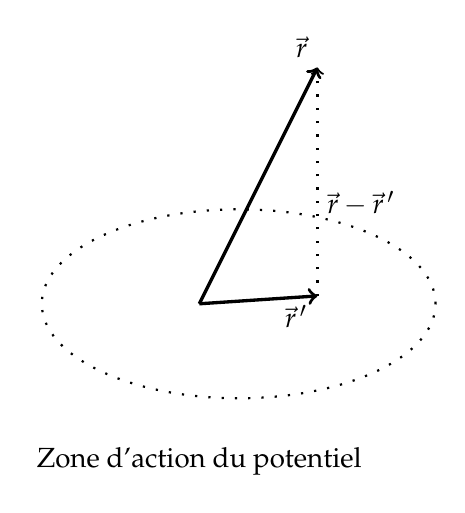
\begin{tikzpicture}
            \coordinate (origin) at (0, 0);
            \coordinate (vec_r) at (1.5, 3);
            \coordinate (vec_r') at (1.5, 0.1);
            
            \draw[black, very thick, ->](0, 0) -- (vec_r);
            \node[align = center, anchor = south east] at (vec_r) {$\vec{r}$};
            
            \draw[black, very thick, ->](0, 0) -- (vec_r');
            \node[align = center, anchor = north east] at (vec_r') {$\pvec{r}'$};
            
            \draw[black, thick, ->, loosely dotted](vec_r') -- (vec_r);
            \node[align = center, anchor = north west] at ($(vec_r')!0.5!(vec_r)$) {$\vec{r} - \pvec{r}'$};
            
            \draw[black, thick, loosely dotted]($(origin) + (0.5, 0)$) ellipse (2.5cm and 1.2cm);
            \node[align = center] at ($(origin) + (0, -2.0)$) {Zone d'action du potentiel};
        \end{tikzpicture}
    \end{figure}
    
    \begin{equation*}
    \begin{split}
        \left\lVert\vec{r} - \pvec{r}'\right\rVert
            &= \sqrt{{r}^{2} - 2 \vec{r} \cdot \pvec{r}' + {r'}^{2}} \\
            &= r \sqrt{1 + {\left(\frac{r'}{r}\right)}^{2} - 2 \frac{\vec{r} \cdot \pvec{r}'}{{r}^{2}}} \\
            &\approx r \sqrt{1 - 2 \frac{\vec{r} \cdot \pvec{r}'}{{r}^{2}}} \\
            &\approx r \left(1 - \frac{\vec{r} \cdot \pvec{r}'}{{r}^{2}}\right)
    \end{split}
    \end{equation*}
    
    \begin{itemize}
        \item
        $\frac{\vec{r}}{r} = {\vec{u}}_{r}$ : vecteur unitaire de la particule diffusée.
        
        \item
        $\left\lVert{\vec{k}}_{f}\right\rVert = \left\lVert{\vec{k}}_{0}\right\rVert$ : diffusion élastique.
    \end{itemize}
    
    \bigskip
    
    D'où :
    
    \begin{equation*}
        {k}_{0} \left\lVert\vec{r} - \pvec{r}'\right\rVert = {k}_{0} r - {k}_{0} \, {\vec{u}}_{r} \cdot \pvec{r}'= {k}_{0} r - {k}_{f} \, {\vec{u}}_{r} \cdot \pvec{r}'
    \end{equation*}
    
    En remplaçant ceci dans l'équation \eqref{chap3_eq/15}, on obtient :
    
    \begin{equation*}
        {\Psi}_{{\vec{k}}_{f}}^{\pm}(\vec{r}) = \frac{{\e}^{\i {\vec{k}}_{0} \cdot \vec{r}}}{(2\pi)^{\frac{3}{2}}} - \frac{m}{2\pi {\hbar}^{2}} \frac{{\e}^{\pm\i {k}_{0} r}}{r} \int {\e}^{\mp\i {k}_{f} \, {\vec{u}}_{r} \cdot \pvec{r}'} V(\pvec{r}') {\Psi}_{{\vec{k}}_{f}}^{\pm}(\pvec{r}') \ {\diff}^{3} r'
    \end{equation*}
    
    Dans ce problème, on ne s'intéresse qu'à l'onde divergente (l'onde sortante ${\Psi}_{{\vec{k}}_{f}}^{+}(\vec{r})$) (Pour qu'il y ait effectivement diffusion).
    
    \begin{equation*}
        {\Psi}_{{\vec{k}}_{f}}^{+}(\vec{r}) = \frac{{\e}^{\i {\vec{k}}_{0} \cdot \vec{r}}}{(2\pi)^{\frac{3}{2}}} - \frac{m}{2\pi {\hbar}^{2}} \frac{{\e}^{\i {k}_{0} r}}{r} \int {\e}^{-\i {k}_{f} \, {\vec{u}}_{r} \cdot \pvec{r}'} V(\pvec{r}') {\Psi}_{{\vec{k}}_{f}}^{+}(\pvec{r}') \ {\diff}^{3} r'
    \end{equation*}
    
    En comparant cette expression à l'expression asymptotique de ${\Psi}_{{\vec{k}}_{f}}(\vec{r})$ : 
    
    \begin{equation*}
        \lim_{r \to \infty} {\Psi}_{{\vec{k}}_{f}}(\vec{r}) \sim \frac{{\e}^{\i {\vec{k}}_{0} \cdot \vec{r}}}{(2\pi)^{\frac{3}{2}}} + \frac{{f}_{{\vec{k}}_{f}}(\theta, \ \phi)}{(2\pi)^{\frac{3}{2}}} \frac{{\e}^{\i {k}_{f} r}}{r}
    \end{equation*}
    
    On obtient l'amplitude de diffusion :
    
    \begin{equation*}
        {f}_{{\vec{k}}_{f}}(\theta, \ \phi) = -\frac{m}{2\pi {\hbar}^{2}} (2\pi)^{\frac{3}{2}} \int {\e}^{-\i {k}_{f} \, {\vec{u}}_{r} \cdot \pvec{r}'} V(\pvec{r}') {\Psi}_{{\vec{k}}_{f}}^{+}(\pvec{r}') \ {\diff}^{3} r'
    \end{equation*}
    
    aussi, les solutions ${\Psi}_{{\vec{k}}_{f}}^{+}(\pvec{r})$ de l'équation intégrale de diffusion sont bien des états stationnaires de diffusion. \\
    
    ${f}_{{\vec{k}}_{f}}(\theta, \ \phi)$ peut aussi s'écrire en notation de \textsc{Dirac} :
    
    \begin{equation*}
        {f}_{{\vec{k}}_{f}}(\theta, \ \phi) = -\frac{m}{2\pi {\hbar}^{2}} (2\pi)^{3} \bra{{\vec{k}}_{f} \vphantom{{\Psi}_{{\vec{k}}_{f}}^{+}}} \opr{V} \ket{{\Psi}_{{\vec{k}}_{f}}^{+}}
    \end{equation*}
    
    et on a la section efficace différentielle :
    
    \begin{equation*}
        \frac{\diff \sigma(\theta, \ \phi)}{\diff \Omega} = {\left\lvert{f}_{{\vec{k}}_{f}}(\theta, \ \phi)\right\rvert}^{2}
    \end{equation*}
    
    \section{Approximation de \textsc{Born}}
    On a déjà vu que :
    
    \begin{equation*}
        \ket{{\Psi}_{{\vec{k}}_{f}}^{+}} = \ket{{\vec{k}}_{0} \vphantom{{\Psi}_{{\vec{k}}_{f}}^{+}}} + {\opr{G}}_{0}^{+}({E}_{0}) \opr{V} \ket{{\Psi}_{{\vec{k}}_{f}}^{+}}
    \end{equation*}
    
    On reécrit $\ket{{\Psi}_{{\vec{k}}_{f}}^{+}}$ en utilisant sa propre équation :
    
    \begin{equation} \label{chap3_eq/19}
    \begin{split}
        \ket{{\Psi}_{{\vec{k}}_{f}}^{+}} 
            &= \ket{{\vec{k}}_{0} \vphantom{{\Psi}_{{\vec{k}}_{f}}^{+}}} + {\opr{G}}_{0}^{+}({E}_{0}) \opr{V} \left(\ket{{\vec{k}}_{0} \vphantom{{\Psi}_{{\vec{k}}_{f}}^{+}}} + {\opr{G}}_{0}^{+}({E}_{0}) \opr{V} \ket{{\Psi}_{{\vec{k}}_{f}}^{+}}\right) \\
            &= \ket{{\vec{k}}_{0} \vphantom{{\Psi}_{{\vec{k}}_{f}}^{+}}} + {\opr{G}}_{0}^{+}({E}_{0}) \opr{V} \ket{{\vec{k}}_{0} \vphantom{{\Psi}_{{\vec{k}}_{f}}^{+}}} + {\opr{G}}_{0}^{+}({E}_{0}) \opr{V} {\opr{G}}_{0}^{+}({E}_{0}) \opr{V} \ket{{\Psi}_{{\vec{k}}_{f}}^{+}} \\
            &= \ket{{\vec{k}}_{0} \vphantom{{\Psi}_{{\vec{k}}_{f}}^{+}}} + {\opr{G}}_{0}^{+}({E}_{0}) \opr{V} \ket{{\vec{k}}_{0} \vphantom{{\Psi}_{{\vec{k}}_{f}}^{+}}} + {\opr{G}}_{0}^{+}({E}_{0}) \opr{V} {\opr{G}}_{0}^{+}({E}_{0}) \opr{V} \ket{{\vec{k}}_{0} \vphantom{{\Psi}_{{\vec{k}}_{f}}^{+}}} + \cdots
    \end{split}
    \end{equation}
    
    La méthode consiste à remplacer dans le second membre l'équation intégrale $\ket{{\Psi}_{{\vec{k}}_{f}}^{+}}$ par son expression initiale, et on répétera cette opération, chaque fois que $\ket{{\Psi}_{{\vec{k}}_{f}}^{+}}$ apparaitra. On obtient une série infinie (appelée série de \textsc{Born}). \\
    
    De même, on aura pour l'amplitude de diffusion : 
    
    \begin{equation*}
    \begin{split}
        {f}_{{\vec{k}}_{f}}(\theta, \ \phi) 
            &= -\frac{m}{2\pi {\hbar}^{2}} (2\pi)^{3} \bra{{\vec{k}}_{f}} \opr{V} \left(\ket{{\vec{k}}_{0}} + {\opr{G}}_{0}^{+}({E}_{0}) \opr{V} \ket{{\vec{k}}_{0}} + {\opr{G}}_{0}^{+}({E}_{0}) \opr{V} {\opr{G}}_{0}^{+}({E}_{0}) \opr{V} \ket{{\vec{k}}_{0}} + \cdots\right) \\
            &= -\frac{m}{2\pi {\hbar}^{2}} (2\pi)^{3} \left(\bra{{\vec{k}}_{f}} \opr{V} \ket{{\vec{k}}_{0}} + \bra{{\vec{k}}_{f}} \opr{V} {\opr{G}}_{0}^{+}({E}_{0}) \opr{V} \ket{{\vec{k}}_{0}} + \cdots\right)
    \end{split}
    \end{equation*}
    
    Dans l'approximation de \textsc{Born}, on remplace $\ket{{\Psi}_{{\vec{k}}_{f}}^{+}}$ par $\ket{{\vec{k}}_{0} \vphantom{{\Psi}_{{\vec{k}}_{f}}^{+}}}$ :
    
    \begin{equation*}
    \begin{split}
        {f}_{{\vec{k}}_{f}}^{\mathcal{B}}(\theta, \ \phi) 
            &= -\frac{m}{2\pi {\hbar}^{2}} (2\pi)^{3} \bra{{\vec{k}}_{f}} \opr{V} \ket{{\vec{k}}_{0}} \\
            &= -\frac{m}{2\pi {\hbar}^{2}} (2\pi)^{3} \bra{{\vec{k}}_{f}} \opr{\identity} \times \opr{V} \times \opr{\identity} \ket{{\vec{k}}_{0}} \\
            &= -\frac{m}{2\pi {\hbar}^{2}} (2\pi)^{3} \iint \bra{{\vec{k}}_{f}} \ket{\vec{r} \vphantom{{\vec{k}}_{f}}} \bra{\vec{r} \vphantom{\pvec{r}'}} \opr{V} \ket{\pvec{r}'} \bra{\pvec{r}' \vphantom{{\vec{k}}_{0}}} \ket{{\vec{k}}_{0}} \ {\diff}^{3} r \, {\diff}^{3} r' \\
            &= -\frac{m}{2\pi {\hbar}^{2}} (2\pi)^{3} \iint \frac{{\e}^{-\i {\vec{k}}_{f} \cdot \vec{r}}}{(2\pi)^{\frac{3}{2}}} \frac{{\e}^{\i {\vec{k}}_{0} \cdot \pvec{r}'}}{(2\pi)^{\frac{3}{2}}} V(\vec{r}, \ \pvec{r}') \ {\diff}^{3} r \, {\diff}^{3} r'
    \end{split}
    \end{equation*}
    
    Pour $V$ local $V(\vec{r}, \ \pvec{r}') = V(\vec{r}) \delta(\vec{r} - \pvec{r}')$ :
    
    \begin{equation*}
        {f}_{{\vec{k}}_{f}}^{\mathcal{B}}(\theta, \ \phi) = -\frac{m}{2\pi {\hbar}^{2}} \int {\e}^{-\i \left({\vec{k}}_{f} - {\vec{k}}_{0}\right) \cdot \vec{r}} V(\vec{r}) \ {\diff}^{3} r
    \end{equation*}
    
    On pose ${\vec{k}}_{f} - {\vec{k}}_{0} = \vec{q}$ : impulsion de transfer
    
    \begin{equation*}
        {f}_{{\vec{k}}_{f}}^{\mathcal{B}}(\theta, \ \phi) = -\frac{m}{2\pi {\hbar}^{2}} \int {\e}^{-\i \vec{q} \cdot \vec{r}} V(\vec{r}) \ {\diff}^{3} r
    \end{equation*}
    
    On peut donner une interprétation physique de la relation \eqref{chap3_eq/19} qui souligne bien l'analogie entre la mécanique quantique et l'optique ondulatoire. En effet, si l'on considère la zone d'action du potentiel comme un milieu diffuseur, on constate que l'onde totale au point $\vec{r}$ donnée par la formule \eqref{chap3_eq/19} correspond à la superposition d'une onde incidente avec une infinité d'ondes provenant de sources secondaires induites dans le milieu diffuseur par l'onde incidente. \\
    
    \begin{remark}
        L'approximation de \textsc{Born} est valable quand le potentiel diffuseur est faible devant l'énergie cinétique de la particule.
    \end{remark}
    
    \section{Diffusion par un potentiel central}
    On a $V(\vec{r}) = V(r, \theta, \phi) = V(\left\lVert\vec{r}\right\rVert) = V(r)$ car on a une symmétrie sphérique. \\
    
    On choisit $\vec{q}$ le long de l'axe $oz$ et on utilise les coordonnées sphériques : 
    
    \begin{figure}[H]
        \centering
        
        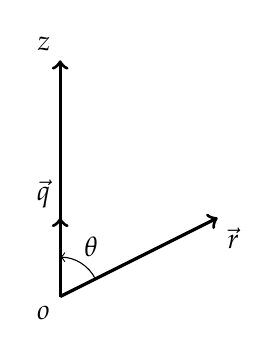
\begin{tikzpicture}
            \coordinate (origin) at (0, 0);
            \coordinate (vec_z) at (0, 3);
            \coordinate (vec_q) at (0, 1);
            \coordinate (vec_r) at (2, 1);
            
            \node[align = center, anchor = north east] at (origin) {$o$};
            
            \draw[black, very thick, ->](0, 0) -- (vec_z);
            \node[align = center, anchor = south east] at (vec_z) {$z$};
            
            \draw[black, very thick, ->](0, 0) -- (vec_q);
            \node[align = center, anchor = south east] at (vec_q) {$\vec{q}$};
            
            \draw[black, very thick, ->](0, 0) -- (vec_r);
            \node[align = center, anchor = north west] at (vec_r) {$\vec{r}$};
            
            \pic[draw, ->, "$\theta$", angle eccentricity = 1.5] {angle = vec_r--origin--vec_q};
        \end{tikzpicture}
    \end{figure}
    
    \begin{align*}
    \begin{split}
        \vec{q} \cdot \vec{r} &= q r \cos{\theta} \\
        {\diff}^{3} r &= {r}^{2} \sin{\theta} \ \diff r \, \diff \theta \, \diff \phi
    \end{split}
    \end{align*}
    
    \begin{equation*}
        {f}_{{\vec{k}}_{f}}^{\mathcal{B}}(\theta, \ \phi) = -\frac{m}{2\pi {\hbar}^{2}} \int_{0}^{\infty} V(r) {r}^{2} \diff r \int_{0}^{2\pi} \diff \phi \int_{0}^{\pi} {\e}^{-\i q r \cos{\theta}} \sin{\theta} \diff \theta
    \end{equation*}
    
    avec :
    
    \begin{equation*}
        \int_{0}^{2\pi} \diff \phi = 2\pi, \qquad \int_{0}^{\pi} {\e}^{-\i q r \cos{\theta}} \sin{\theta} \diff \theta = 2 \frac{\sin{q r}}{q r}
    \end{equation*}
    
    D'où :
    
    \begin{equation*}
        {f}_{{\vec{k}}_{f}}^{\mathcal{B}}(\theta, \ \phi) = -\frac{2m}{{\hbar}^{2}} \frac{1}{q} \int_{0}^{\infty} V(r) r \sin{q r} \ \diff r
    \end{equation*}
    
    \bigskip
    
    \begin{application}
        \leavevmode
        
        \begin{itemize}
            \itemsep2em
            
            \item 
            Potentiel de \textsc{Yukawa} : $\qquad V(r) = {V}_{0} \frac{{\e}^{- \alpha r}}{r} \quad (\alpha > 0)$
            
            \begin{equation*}
            \begin{split}
                {f}_{{\vec{k}}_{f}}^{\mathcal{B}}(\theta, \ \phi) 
                    &= -\frac{2m}{{\hbar}^{2}} \frac{{V}_{0}}{q} \int_{0}^{\infty} {\e}^{- \alpha r} \sin{q r} \ \diff r \\
                    &= -\frac{2m}{{\hbar}^{2}} \frac{{V}_{0}}{q} \Im \int_{0}^{\infty} {\e}^{(- \alpha + \i q) r} \ \diff r \\
                    &= -\frac{2m}{{\hbar}^{2}} \frac{{V}_{0}}{{\alpha}^{2} + {q}^{2}} 
            \end{split}
            \end{equation*}
            
            \item
            Diffusion élastique :
            
            \begin{figure}[H]
                \centering
                
                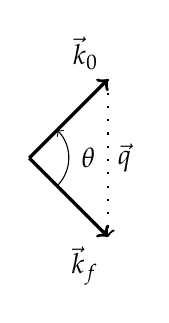
\begin{tikzpicture}
                    \coordinate (origin) at (0, 0);
                    \coordinate (vec_k0) at (1, 1);
                    \coordinate (vec_kf) at (1, -1);
                    
                    \draw[black, very thick, ->](0, 0) -- (vec_k0);
                    \node[align = center, anchor = south east] at (vec_k0) {${\vec{k}}_{0}$};
                    
                    \draw[black, very thick, ->](0, 0) -- (vec_kf);
                    \node[align = center, anchor = north east] at (vec_kf) {${\vec{k}}_{f}$};
                    
                    \draw[black, thick, ->, loosely dotted](vec_k0) -- (vec_kf);
                    \node[align = center, anchor = west] at ($(vec_kf)!0.5!(vec_k0)$) {$\vec{q}$};
                    
                    \pic[draw, ->, "$\theta$", angle eccentricity = 1.5] {angle = vec_kf--origin--vec_k0};
                \end{tikzpicture}
            \end{figure}
            
            \begin{equation*}
                \left\lVert{\vec{k}}_{f}\right\rVert = \left\lVert{\vec{k}}_{0}\right\rVert \implies q = 2 {k}_{0} \sin{\frac{\theta}{2}} \quad \left(\theta \ \text{est l'angle de diffusion}\right)
            \end{equation*}
            
            \begin{equation*}
                {f}_{{\vec{k}}_{f}}^{\mathcal{B}}(\theta, \ \phi) = -\frac{2m}{{\hbar}^{2}} \frac{{V}_{0}}{{\alpha}^{2} + 4 {k}_{0}^{2} \sin^{2} \frac{\theta}{2}}
            \end{equation*}
            
            \item 
            Diffusion Coulombienne : $\qquad V(r) = -\frac{Z {e}^{2}}{r}$ \\
            (Potentiel de \textsc{Yukawa} pour $\alpha = 0$ et ${V}_{0} = -Z {e}^{2}$)
            
            \begin{equation*}
                {f}_{{\vec{k}}_{f}}^{\mathcal{B}}(\theta, \ \phi) = \frac{2m}{{\hbar}^{2}} \frac{Z {e}^{2}}{4 {k}_{0}^{2} \sin^{2} \frac{\theta}{2}}
            \end{equation*}
            
            on pose ${k}_{0}^{2} = \frac{2m {E}_{0}}{{\hbar}^{2}}$ :
            
            \begin{equation*}
                {f}_{{\vec{k}}_{f}}^{\mathcal{B}}(\theta, \ \phi) = \frac{Z {e}^{2}}{4 {E}_{0} \sin^{2} \frac{\theta}{2}}, \qquad \frac{\diff \sigma(\theta, \ \phi)}{\diff \Omega} = \frac{{Z}^{2} {e}^{4}}{16 {E}_{0}^{4} \sin^{4} \frac{\theta}{2}}
            \end{equation*}
            
            C'est la formule de \textsc{Rutherford}.
            
        \end{itemize}
    \end{application}
    
    \section{Équation de \textsc{Lippmann-Schwinger}}
    On a déjà trouvé l'équation intégrale :
    
    \begin{equation*}
        \ket{{\Psi}_{{\vec{k}}_{f}}^{+}} = \ket{{\vec{k}}_{0} \vphantom{{\Psi}_{{\vec{k}}_{f}}^{+}}} + {\opr{G}}_{0}^{+}({E}_{0}) \opr{V} \ket{{\Psi}_{{\vec{k}}_{f}}^{+}}, \qquad {\opr{G}}_{0}^{+}({E}_{0}) = \frac{1}{{E}_{0} - {\opr{H}}_{0}}
    \end{equation*}
    
    Afin d'éviter les problèmes de singularité, on prend : 
    
    \begin{equation*}
    \begin{split}
        {\opr{G}}_{0}^{+}(E) 
        &= \frac{1}{{E}_{0} - {\opr{H}}_{0} + \i \varepsilon}, \qquad \varepsilon \to 0 \\
        &= \frac{1}{E - {\opr{H}}_{0}}, \qquad\qquad \ E = {E}_{0} + \i \varepsilon
    \end{split}
    \end{equation*}
    
    Ce qui donne l'équation :
    
    \begin{equation*}
        \ket{{\Psi}_{{\vec{k}}_{f}}^{+}} = \ket{{\vec{k}}_{0} \vphantom{{\Psi}_{{\vec{k}}_{f}}^{+}}} + {\opr{G}}_{0}^{+}(E) \opr{V} \ket{{\Psi}_{{\vec{k}}_{f}}^{+}}
    \end{equation*}
    
    Connu par l'équation de \textsc{Lippmann-Schwinger}. Si on applique $E - {\opr{H}}_{0}$ à $\ket{{\Psi}_{{\vec{k}}_{f}}^{+}}$, tel que :
    
    \begin{equation*}
    \begin{split}
        \left(E - {\opr{H}}_{0}\right) \ket{{\Psi}_{{\vec{k}}_{f}}^{+}} 
            &= \left(E - {\opr{H}}_{0}\right) \ket{{\vec{k}}_{0} \vphantom{{\Psi}_{{\vec{k}}_{f}}^{+}}} + \underbrace{\left(E - {\opr{H}}_{0}\right) {\opr{G}}_{0}^{+}(E)}_{\opr{\identity}} \opr{V} \ket{{\Psi}_{{\vec{k}}_{f}}^{+}} \\
            &= \left(E - {\opr{H}}_{0}\right) \ket{{\vec{k}}_{0} \vphantom{{\Psi}_{{\vec{k}}_{f}}^{+}}} + \opr{V} \ket{{\Psi}_{{\vec{k}}_{f}}^{+}} \\
    \end{split}
    \end{equation*}
    
    On regroupe les termes en $\ket{{\Psi}_{{\vec{k}}_{f}}^{+}}$ :
    
    \begin{equation*}
    \begin{split}
        \left(E - {\opr{H}}_{0} - \opr{V}\right) \ket{{\Psi}_{{\vec{k}}_{f}}^{+}} 
            &= \left(E - {\opr{H}}_{0}\right) \ket{{\vec{k}}_{0} \vphantom{{\Psi}_{{\vec{k}}_{f}}^{+}}} \\
            &= \left(E - {\opr{H}}_{0} - \opr{V}\right) \ket{{\vec{k}}_{0} \vphantom{{\Psi}_{{\vec{k}}_{f}}^{+}}} + \opr{V} \ket{{\vec{k}}_{0} \vphantom{{\Psi}_{{\vec{k}}_{f}}^{+}}}
    \end{split}
    \end{equation*}
    
    \begin{equation*}
    \begin{split}
        \implies \ket{{\Psi}_{{\vec{k}}_{f}}^{+}}
            &= \ket{{\vec{k}}_{0} \vphantom{{\Psi}_{{\vec{k}}_{f}}^{+}}} + \frac{1}{E - {\opr{H}}_{0} - \opr{V}} \opr{V} \ket{{\vec{k}}_{0} \vphantom{{\Psi}_{{\vec{k}}_{f}}^{+}}} \\
            &= \ket{{\vec{k}}_{0} \vphantom{{\Psi}_{{\vec{k}}_{f}}^{+}}} + \frac{1}{{E}_{0} - \opr{H} + \i \varepsilon} \opr{V} \ket{{\vec{k}}_{0} \vphantom{{\Psi}_{{\vec{k}}_{f}}^{+}}}, \qquad \opr{H} = {\opr{H}}_{0} + \opr{V}
    \end{split}
    \end{equation*}
    
    Cette dernière expression fait intervenir l'Hamiltonien avec interaction : $\opr{H} = {\opr{H}}_{0} + \opr{V}$ \\
    
    Par conséquent, l'état stationnaire de diffusion $\ket{{\Psi}_{{\vec{k}}_{f}}^{+}}$ qui satisfait l'équation de \textsc{Lippmann-Schwinger} vérifie aussi cette 2\up{ème} forme.
    
    \subsection{Opérateur ou matrice de transition}
    On appelle $\opr{T}$ l'opérateur de transition, l'opérateur vérifier la relation suivante :
    
    \begin{equation*}
        \opr{T} \ket{{\vec{k}}_{0} \vphantom{{\Psi}_{{\vec{k}}_{f}}^{+}}} = \opr{V} \ket{{\Psi}_{{\vec{k}}_{f}}^{+}}
    \end{equation*}
    
    En introduisant la 1\up{ère} expression de $\ket{{\Psi}_{{\vec{k}}_{f}}^{+}}$  dans le second membre :
    
    \begin{equation*}
    \begin{split}
        \opr{T} \ket{{\vec{k}}_{0} \vphantom{{\Psi}_{{\vec{k}}_{f}}^{+}}} 
            &= \opr{V} \ket{{\vec{k}}_{0} \vphantom{{\Psi}_{{\vec{k}}_{f}}^{+}}} + \opr{V} {\opr{G}}_{0}^{+}(E) \opr{V} \ket{{\Psi}_{{\vec{k}}_{f}}^{+}} \\
            &= \opr{V} \ket{{\vec{k}}_{0} \vphantom{{\Psi}_{{\vec{k}}_{f}}^{+}}} + \opr{V} {\opr{G}}_{0}^{+}(E) \opr{T} \ket{{\vec{k}}_{0} \vphantom{{\Psi}_{{\vec{k}}_{f}}^{+}}} \\
            &= \left(\opr{V} + \opr{V} {\opr{G}}_{0}^{+}(E) \opr{T}\right) \ket{{\vec{k}}_{0} \vphantom{{\Psi}_{{\vec{k}}_{f}}^{+}}}
    \end{split}
    \end{equation*}
    
    D'où $\opr{T} = \opr{V} + \opr{V} {\opr{G}}_{0}^{+}(E) \opr{T}$, c'est la 3\up{ème} forme de l'équation de \textsc{Lippmann-Schwinger}. \\
    
    De même, en introduisant la 2\up{ème} expression de $\ket{{\Psi}_{{\vec{k}}_{f}}^{+}}$  dans le second membre :
    
    \begin{equation*}
    \begin{split}
        \opr{T} \ket{{\vec{k}}_{0} \vphantom{{\Psi}_{{\vec{k}}_{f}}^{+}}}
            &= \opr{V} \ket{{\vec{k}}_{0} \vphantom{{\Psi}_{{\vec{k}}_{f}}^{+}}} + \opr{V} \frac{1}{{E}_{0} - \opr{H} + \i \varepsilon} \opr{V} \ket{{\vec{k}}_{0} \vphantom{{\Psi}_{{\vec{k}}_{f}}^{+}}} \\
            &= \left(\opr{V} + \opr{V} {\opr{G}}^{+}(E) \opr{V}\right) \ket{{\vec{k}}_{0} \vphantom{{\Psi}_{{\vec{k}}_{f}}^{+}}}, \qquad {\opr{G}}^{+}(E) = \frac{1}{{E}_{0} - \opr{H} + \i \varepsilon}
    \end{split}
    \end{equation*}
    
    On obtient la 4\up{ème} forme de l'équation de \textsc{Lippmann-Schwinger}, avec $\opr{T} = \opr{V} + \opr{V} {\opr{G}}^{+}(E) \opr{V}$.
    
    \subsection{Développement de \textsc{Born}}
    Le développement de \textsc{Born} consiste à réinjecter l'expression de $\opr{T}$ auto-cohérente un certain nombre de fois, on obtient donc successivement :
    
    \begin{equation*}
    \begin{split}
        \opr{T}
            &= \opr{V} + \opr{V} {\opr{G}}_{0}^{+}(E) \opr{T} \\
            &= \opr{V} + \opr{V} {\opr{G}}_{0}^{+}(E) \left(\opr{V} + \opr{V} {\opr{G}}_{0}^{+}(E) \opr{T}\right) \\
            &= \opr{V} + \opr{V} {\opr{G}}_{0}^{+}(E) \opr{V} + \opr{V} {\opr{G}}_{0}^{+}(E)\opr{V} {\opr{G}}_{0}^{+}(E) \opr{T} \\
            &= \opr{V} + \opr{V} {\opr{G}}_{0}^{+}(E) \opr{V} + \opr{V} {\opr{G}}_{0}^{+}(E)\opr{V} {\opr{G}}_{0}^{+}(E) \opr{V} + \cdots
    \end{split}
    \end{equation*}

    Pour que la série converge vite, $V$ doit être faible devant l'énergie initial ${E}_{0}$ ($V \ll {E}_{0}$).
    
    \subsection{L'amplitude de diffusion en fonction de \texorpdfstring{$\opr{T}$}{T}}
    On a déjà trouvé :
    
    \begin{equation*}
        {f}_{{\vec{k}}_{f}}(\theta, \ \phi) = -\frac{m}{{\hbar}^{2}} (2\pi)^{2} \bra{{\vec{k}}_{f} \vphantom{{\Psi}_{{\vec{k}}_{f}}^{+}}} \opr{V} \ket{{\Psi}_{{\vec{k}}_{f}}^{+}}
    \end{equation*}
    
    Or selon la définition de $\opr{T}$ :
    
    \begin{equation*}
        \opr{T} \ket{{\vec{k}}_{0} \vphantom{{\Psi}_{{\vec{k}}_{f}}^{+}}} = \opr{V} \ket{{\Psi}_{{\vec{k}}_{f}}^{+}}
    \end{equation*}
    
    Alors :
    
    \begin{equation*}
        {f}_{{\vec{k}}_{f}}(\theta, \ \phi) = -\frac{m}{{\hbar}^{2}} (2\pi)^{2} \bra{{\vec{k}}_{f} \vphantom{{\Psi}_{{\vec{k}}_{f}}^{+}}} \opr{T} \ket{{\vec{k}}_{0} \vphantom{{\Psi}_{{\vec{k}}_{f}}^{+}}}
    \end{equation*}
    
    au 1\up{ère} ordre : $\opr{T} = \opr{V}$
    
    \begin{equation*}
    \begin{split}
        {f}_{{\vec{k}}_{f}}^{\mathcal{B}}(\theta, \ \phi) 
            &= -\frac{m}{{\hbar}^{2}} (2\pi)^{2} \bra{{\vec{k}}_{f} \vphantom{{\Psi}_{{\vec{k}}_{f}}^{+}}} \opr{V} \ket{{\vec{k}}_{0} \vphantom{{\Psi}_{{\vec{k}}_{f}}^{+}}} \\
            &= -\frac{m}{{\hbar}^{2}} \frac{(2\pi)^{2}}{(2\pi)^{3}} \int {\e}^{-\i {\vec{k}}_{f} \cdot \vec{r}} V(\vec{r}) {\e}^{\i {\vec{k}}_{0} \cdot \vec{r}} \ {\diff}^{3} r \\
            &= -\frac{m}{{\hbar}^{2}} \frac{1}{2\pi} \int {\e}^{-\i \left({\vec{k}}_{f} - {\vec{k}}_{0}\right) \cdot \vec{r}} V(\vec{r}) \ {\diff}^{3} r \\
    \end{split}
    \end{equation*}
    
    On pose ${\vec{k}}_{f} - {\vec{k}}_{0} = \vec{q}$ :
    
    \begin{equation*}
        {f}_{{\vec{k}}_{f}}^{\mathcal{B}}(\theta, \ \phi) = -\frac{m}{2\pi {\hbar}^{2}} \int {\e}^{-\i \vec{q} \cdot \vec{r}} V(\vec{r}) \ {\diff}^{3} r
    \end{equation*}
    
    Dans le cas d'un potentiel central $V(\vec{r}) = V(r)$, on trouve :
    
    \begin{equation*}
    \begin{split}
        {f}_{{\vec{k}}_{f}}^{\mathcal{B}}(\theta, \ \phi)
            &= -\frac{m}{2\pi {\hbar}^{2}} \int_{0}^{\infty} V(r) {r}^{2} \diff r \int_{0}^{2\pi} \diff \phi \int_{0}^{\pi} {\e}^{-\i q r \cos{\theta}} \sin{\theta} \diff \theta \\
            &= -\frac{m}{2\pi {\hbar}^{2}} \int_{0}^{\infty} V(r) {r}^{2} \diff r \int_{0}^{2\pi} \diff \phi \int_{-1}^{+1} {\e}^{-\i q r \cos{\theta}} \diff \cos{\theta} \\
            &= -\frac{2m}{{\hbar}^{2}} \int_{0}^{\infty} V(r) {r}^{2} \frac{\sin{q r}}{q r} \ \diff r
    \end{split}
    \end{equation*}
    
    Si $q \to 0$, alors $\frac{\sin{q r}}{q r} \to 1$, d'où :
    
    \begin{equation*}
        {f}_{{\vec{k}}_{f}}^{\mathcal{B}}(\theta, \ \phi) = -\frac{2m}{{\hbar}^{2}} \int_{0}^{\infty} V(r) {r}^{2} \ \diff r
    \end{equation*}
    
\end{document}